\addcontentsline{toc}{chapter}{LAMPIRAN}
\appendix 
\chapter{Transkrip Percakapan}
\begin{flushleft}
Hari: Jumat
\linebreak
Tanggal: 24 Februari 2023
\linebreak
PL: Penulis
\linebreak
N: Narasumber
\linebreak
\linebreak
PL: Bagaimana cara kerja sistem aplikasi pengkajian luka ini?
\linebreak
N: Kita akan membuat aplikasi pengkajian luka yang berjalan di android dan membantu perawat dalam mengkaji luka kronis pasien.
\linebreak
PL: Untuk saat ini sejauh mana aplikasi ini berjalan?
\linebreak
N: Untuk saat ini, sistem ini sudah berjalan hingga mendapatkan data kajian berupa gambar.
\linebreak
PL: Apakah masih ada kelemahan pada aplikasi ini?
\linebreak
N: Karena aplikasi ini masih hanya menyimpan data kajian yang berupa gambar, maka data kajian yang lainnya belum lengkap. Dan oleh sebab itu, lebih baik dilanjutkan dengan menyimpan seluruh data kajian luka dan diletakkan pada medical record pasien agar perawat mudah dalam melihat riwayat kondisi pasien.
\linebreak
PL: Bagaimana prioritas dalam menentukan data kajian luka tersebut?
\linebreak
N: Saya menganjurkan untuk menggunakan Bates-Jensen karena lebih lengkap dalam melakukan kajian luka.
\linebreak
PL: Bagaimana manajemen keperawatan?
\linebreak
N: Pada saat pertama kali pasien datang langsung didata status pasien secara lengkap. Lalu dilanjutkan dengan pengkajian umum luka dan pengkajian lokal luka. Nah setelah itu Dicatat perkembangan dan tujuan keperawatannya mau kemana. Apabila ada tindakan yang perlu dilakukan terhadap pasien nanti perawat meminta persetujuan pasien untuk dapat melakukan tindakan pengobatan. Dan diakhiri dengan mencatat rekap kunjungan secara ringkas.
\linebreak
PL: Mengapa pasien perlu mendapat data kajian miliknya pribadi?
\linebreak
N: Karena pasien harus melihat progres penyembuhan setelah mendapat pengobatan agar dapat menilai sendiri dan membantu perawat dalam memutuskan tindakan selanjutnya.
\linebreak.
\end{flushleft}

\chapter{\emph{Bates-Jensen Wound Assessment Tools}}

\begin{figure}[H]
	\centering
	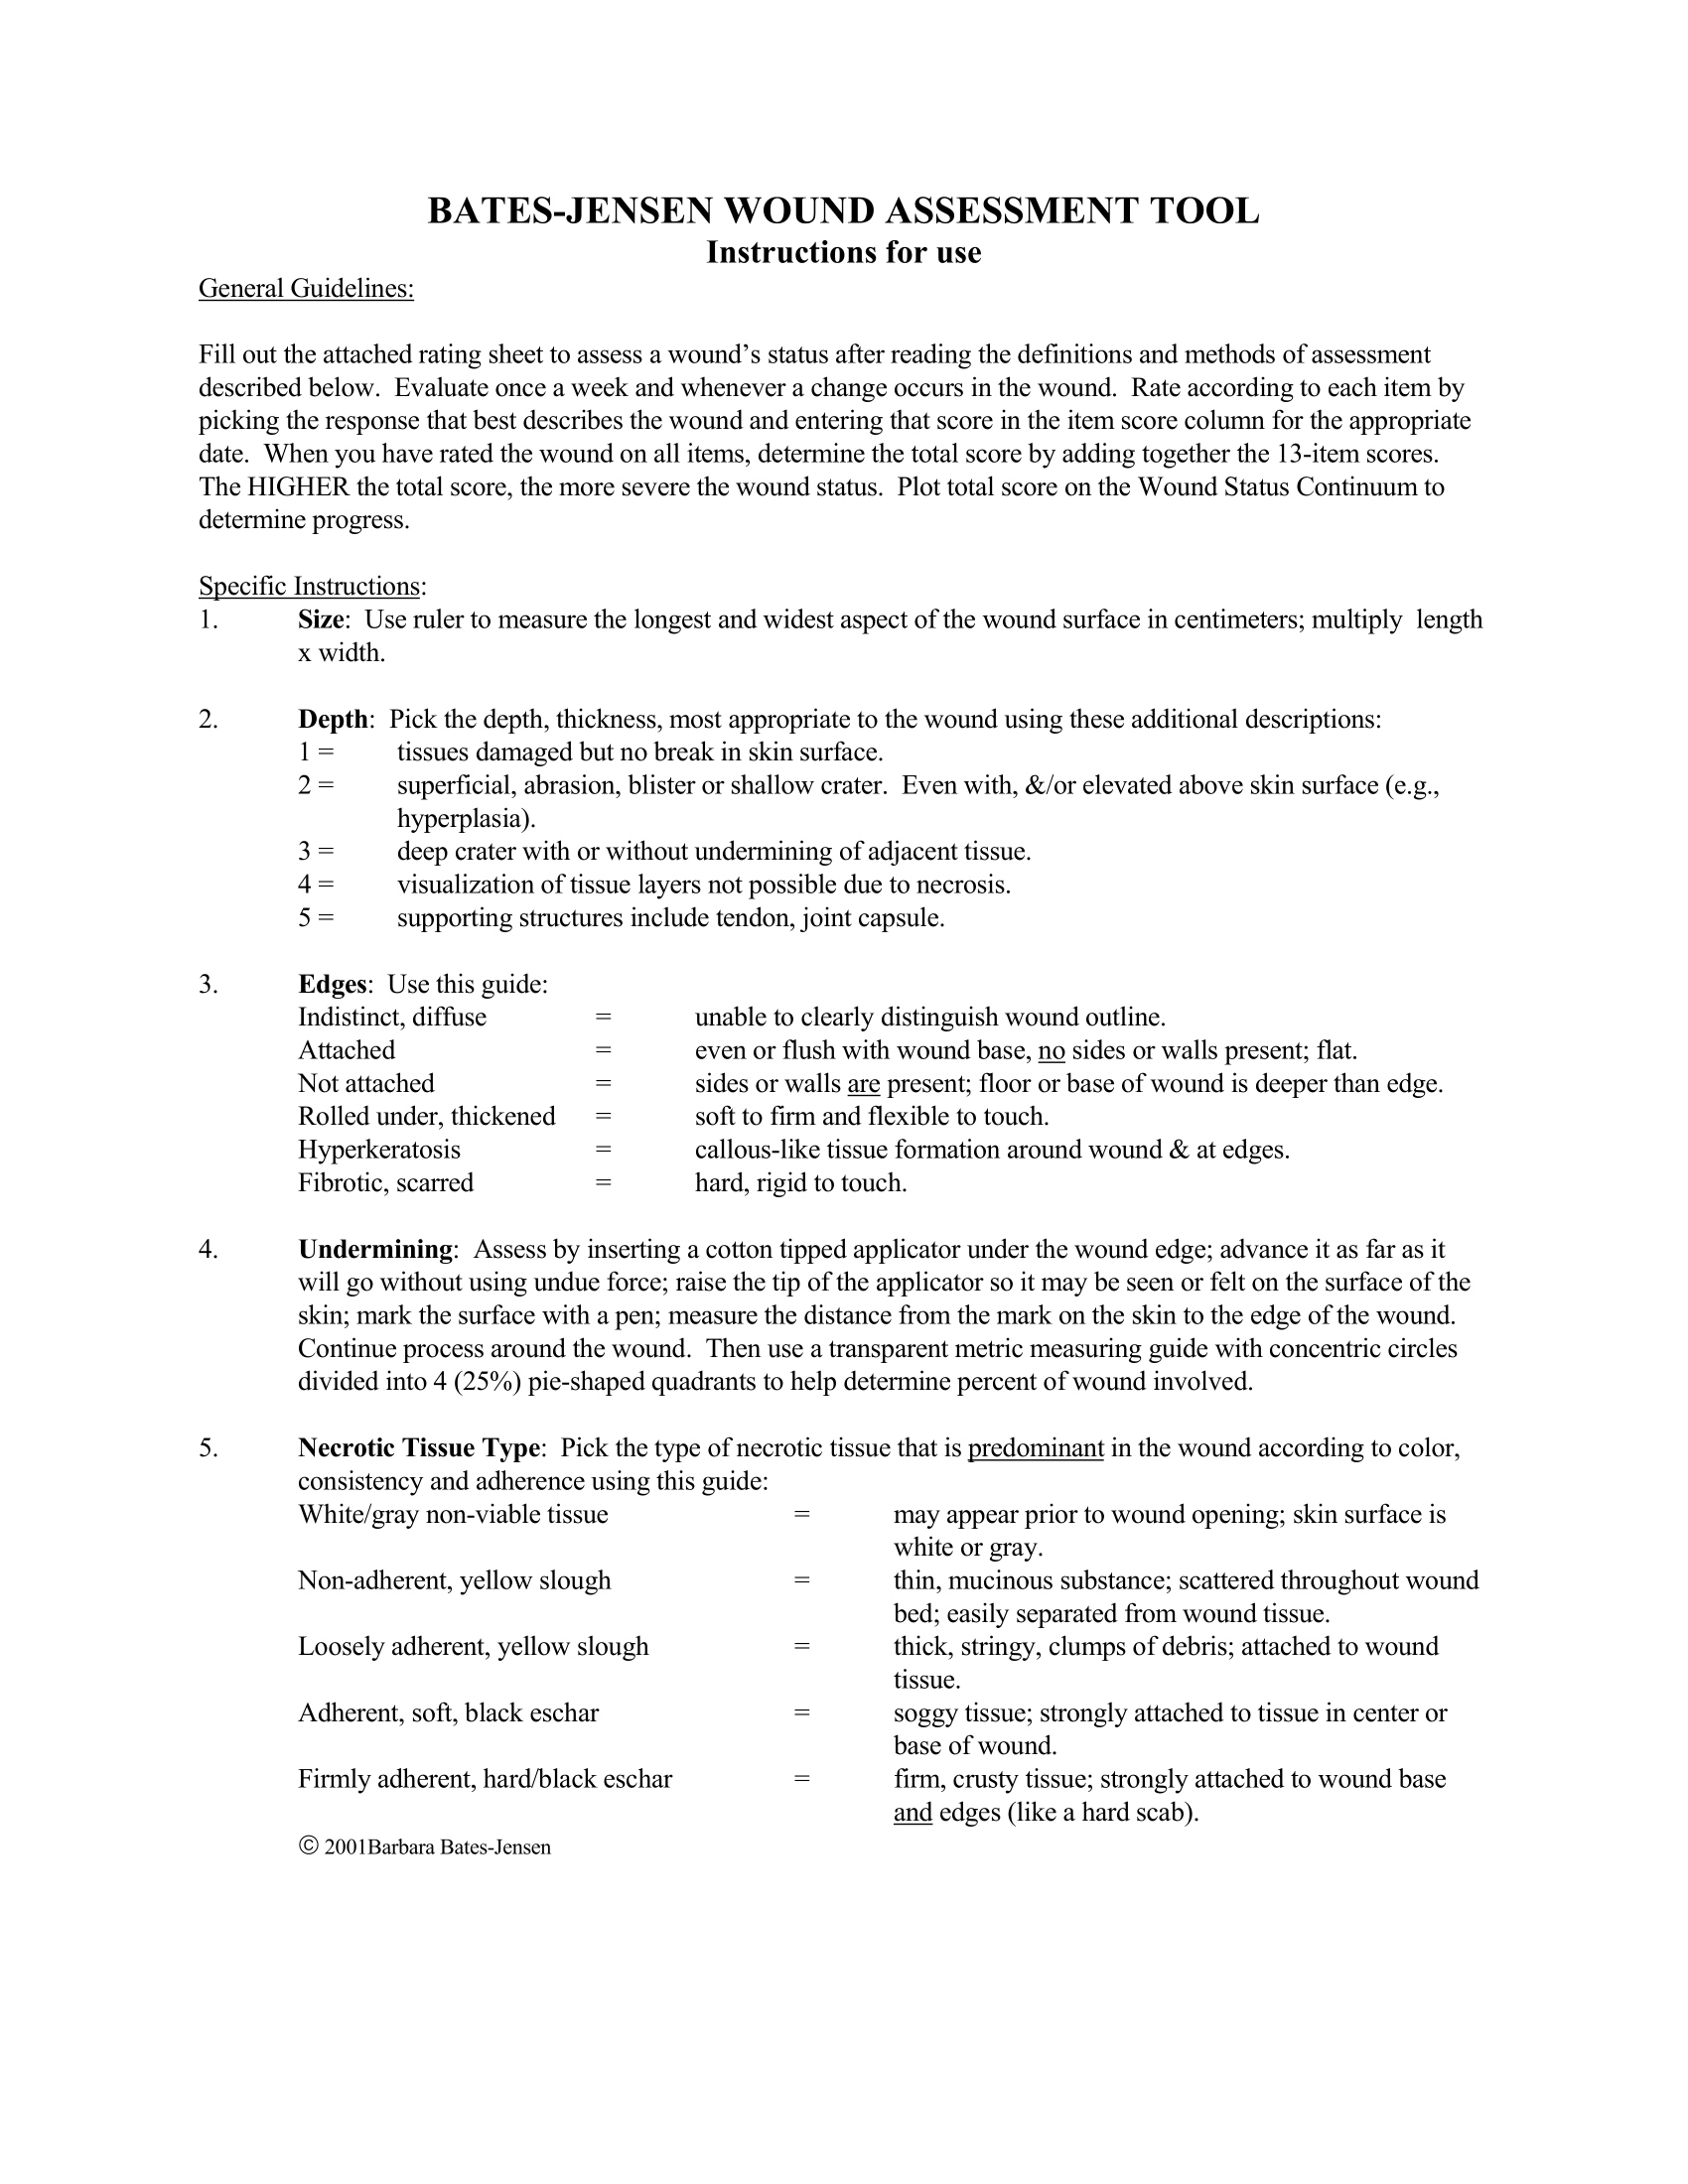
\includegraphics[keepaspectratio, width=14cm]{gambar/BWAT-1}
	\label{gambar:bwat_1}
\end{figure}

\begin{figure}[H]
	\centering
	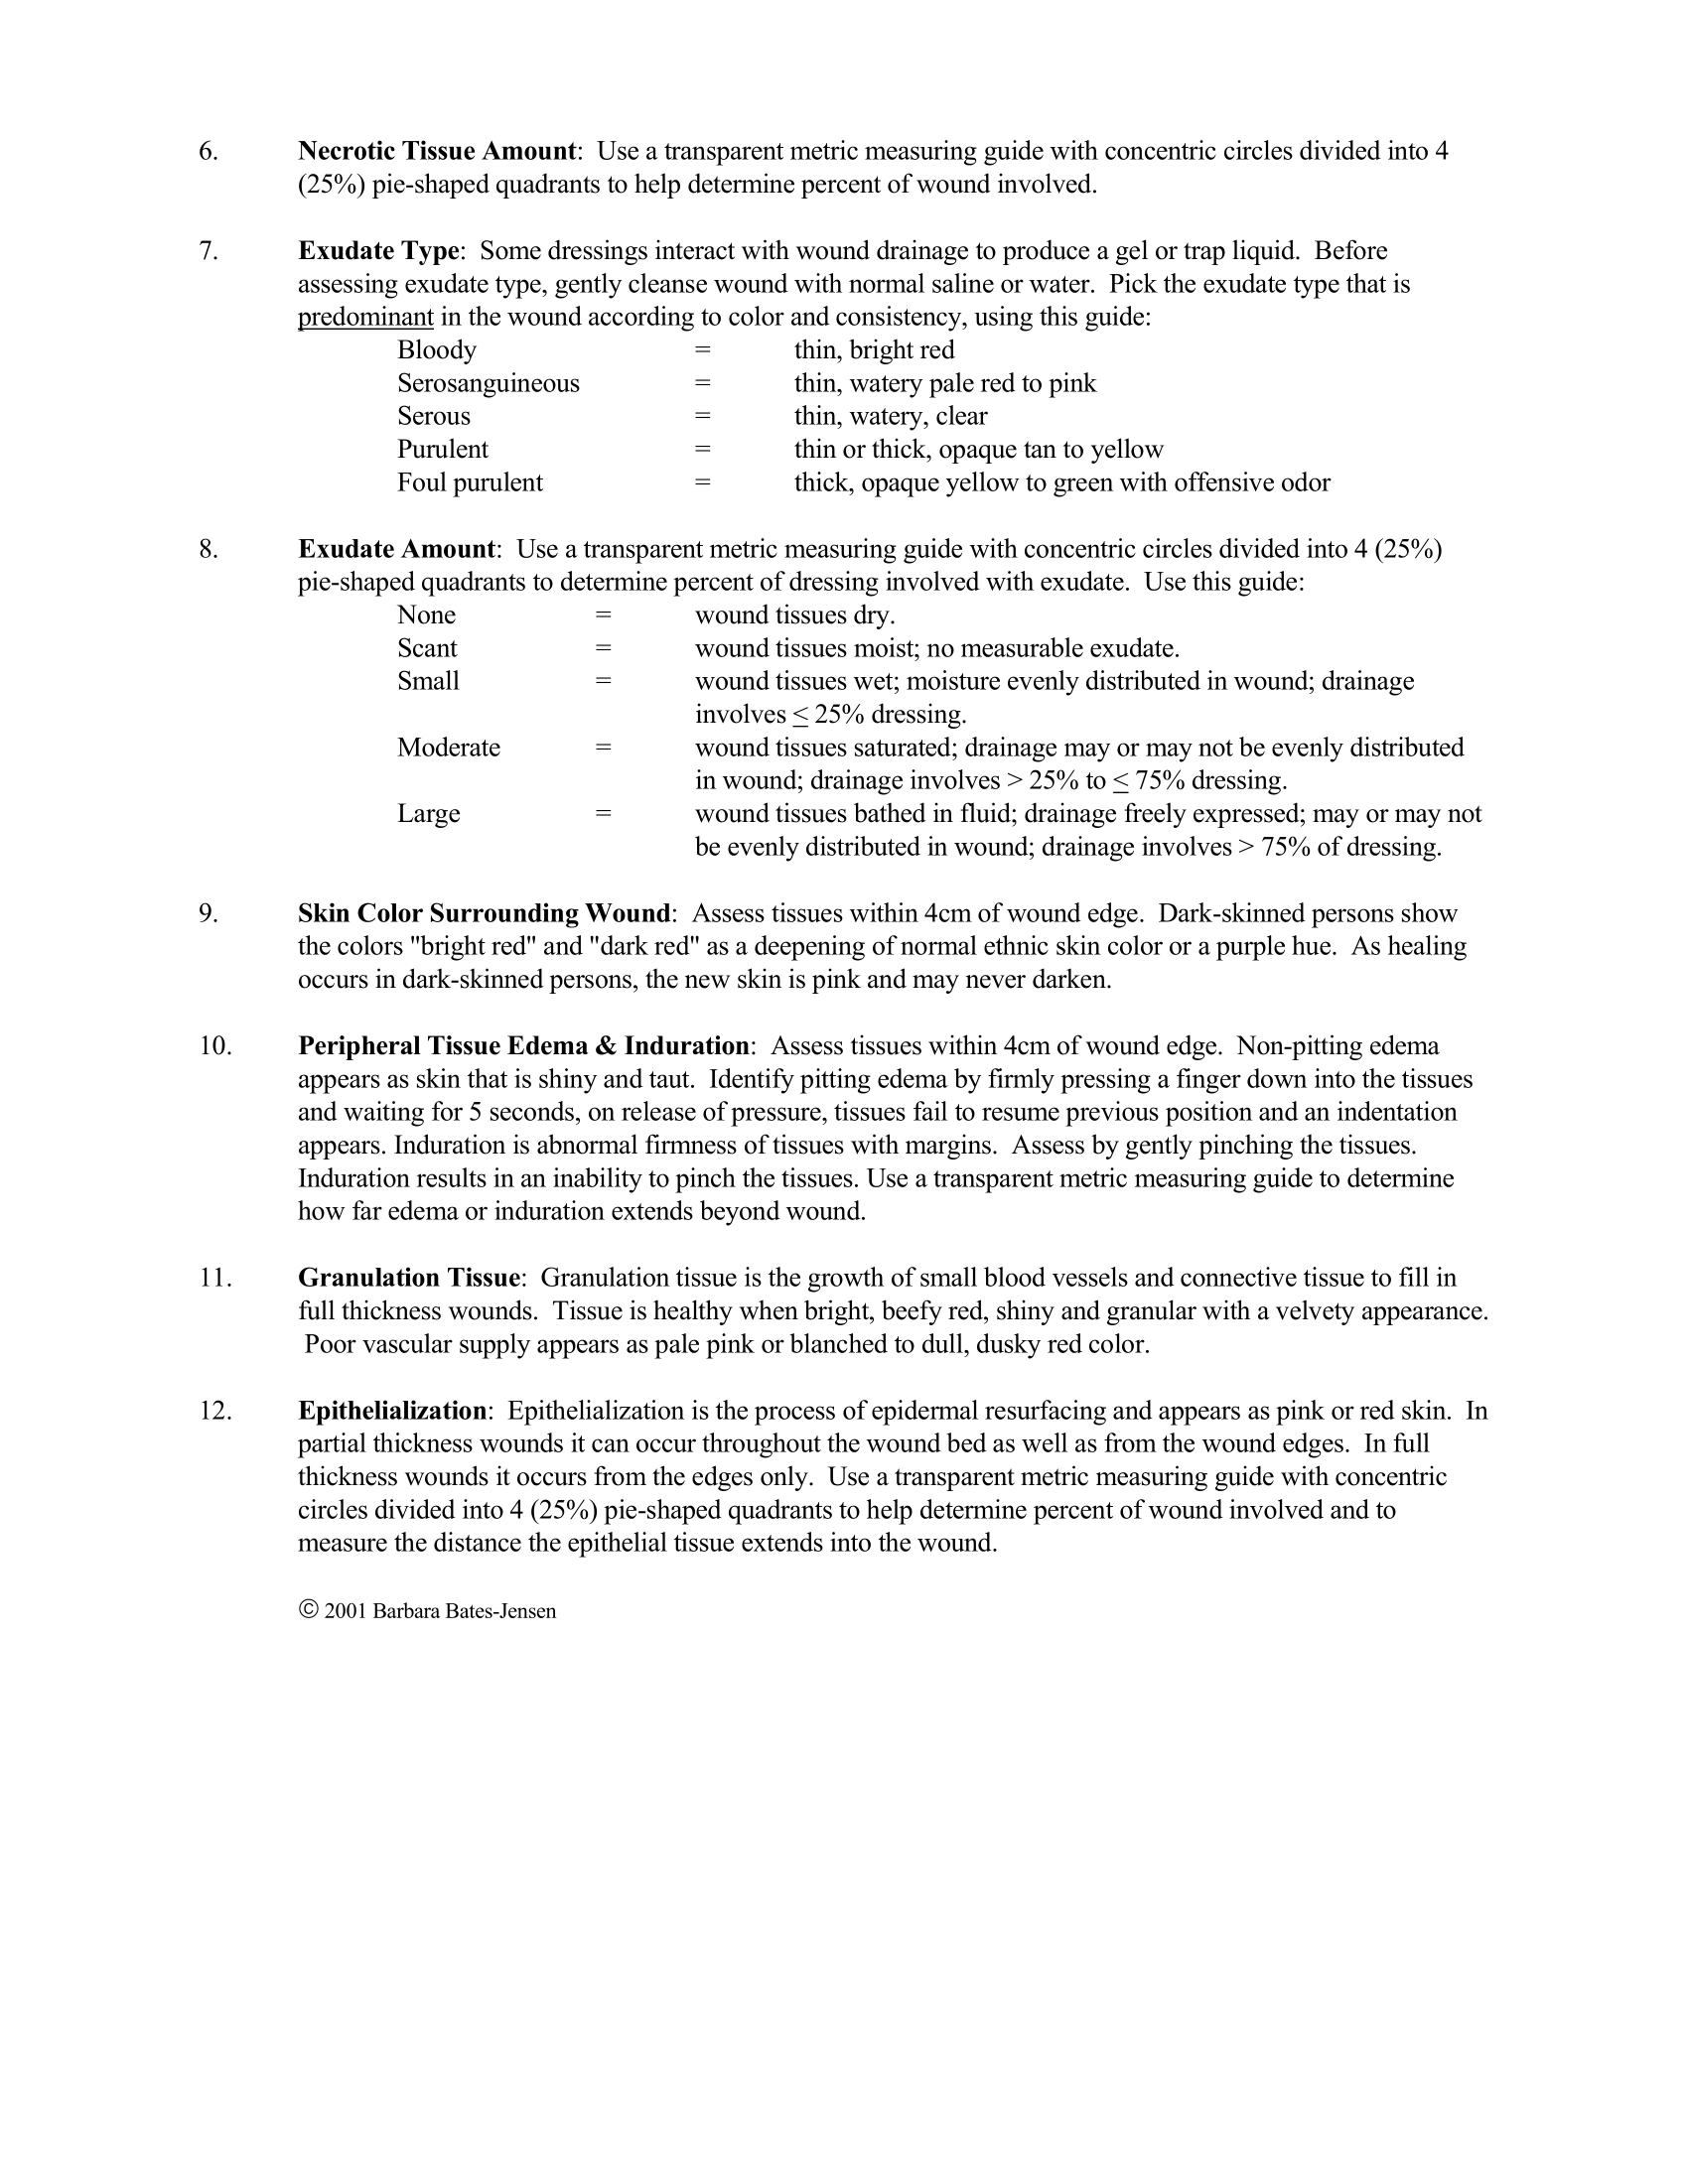
\includegraphics[keepaspectratio, width=14cm]{gambar/BWAT-2}
	\label{gambar:bwat_2}
\end{figure}

\begin{figure}[H]
	\centering
	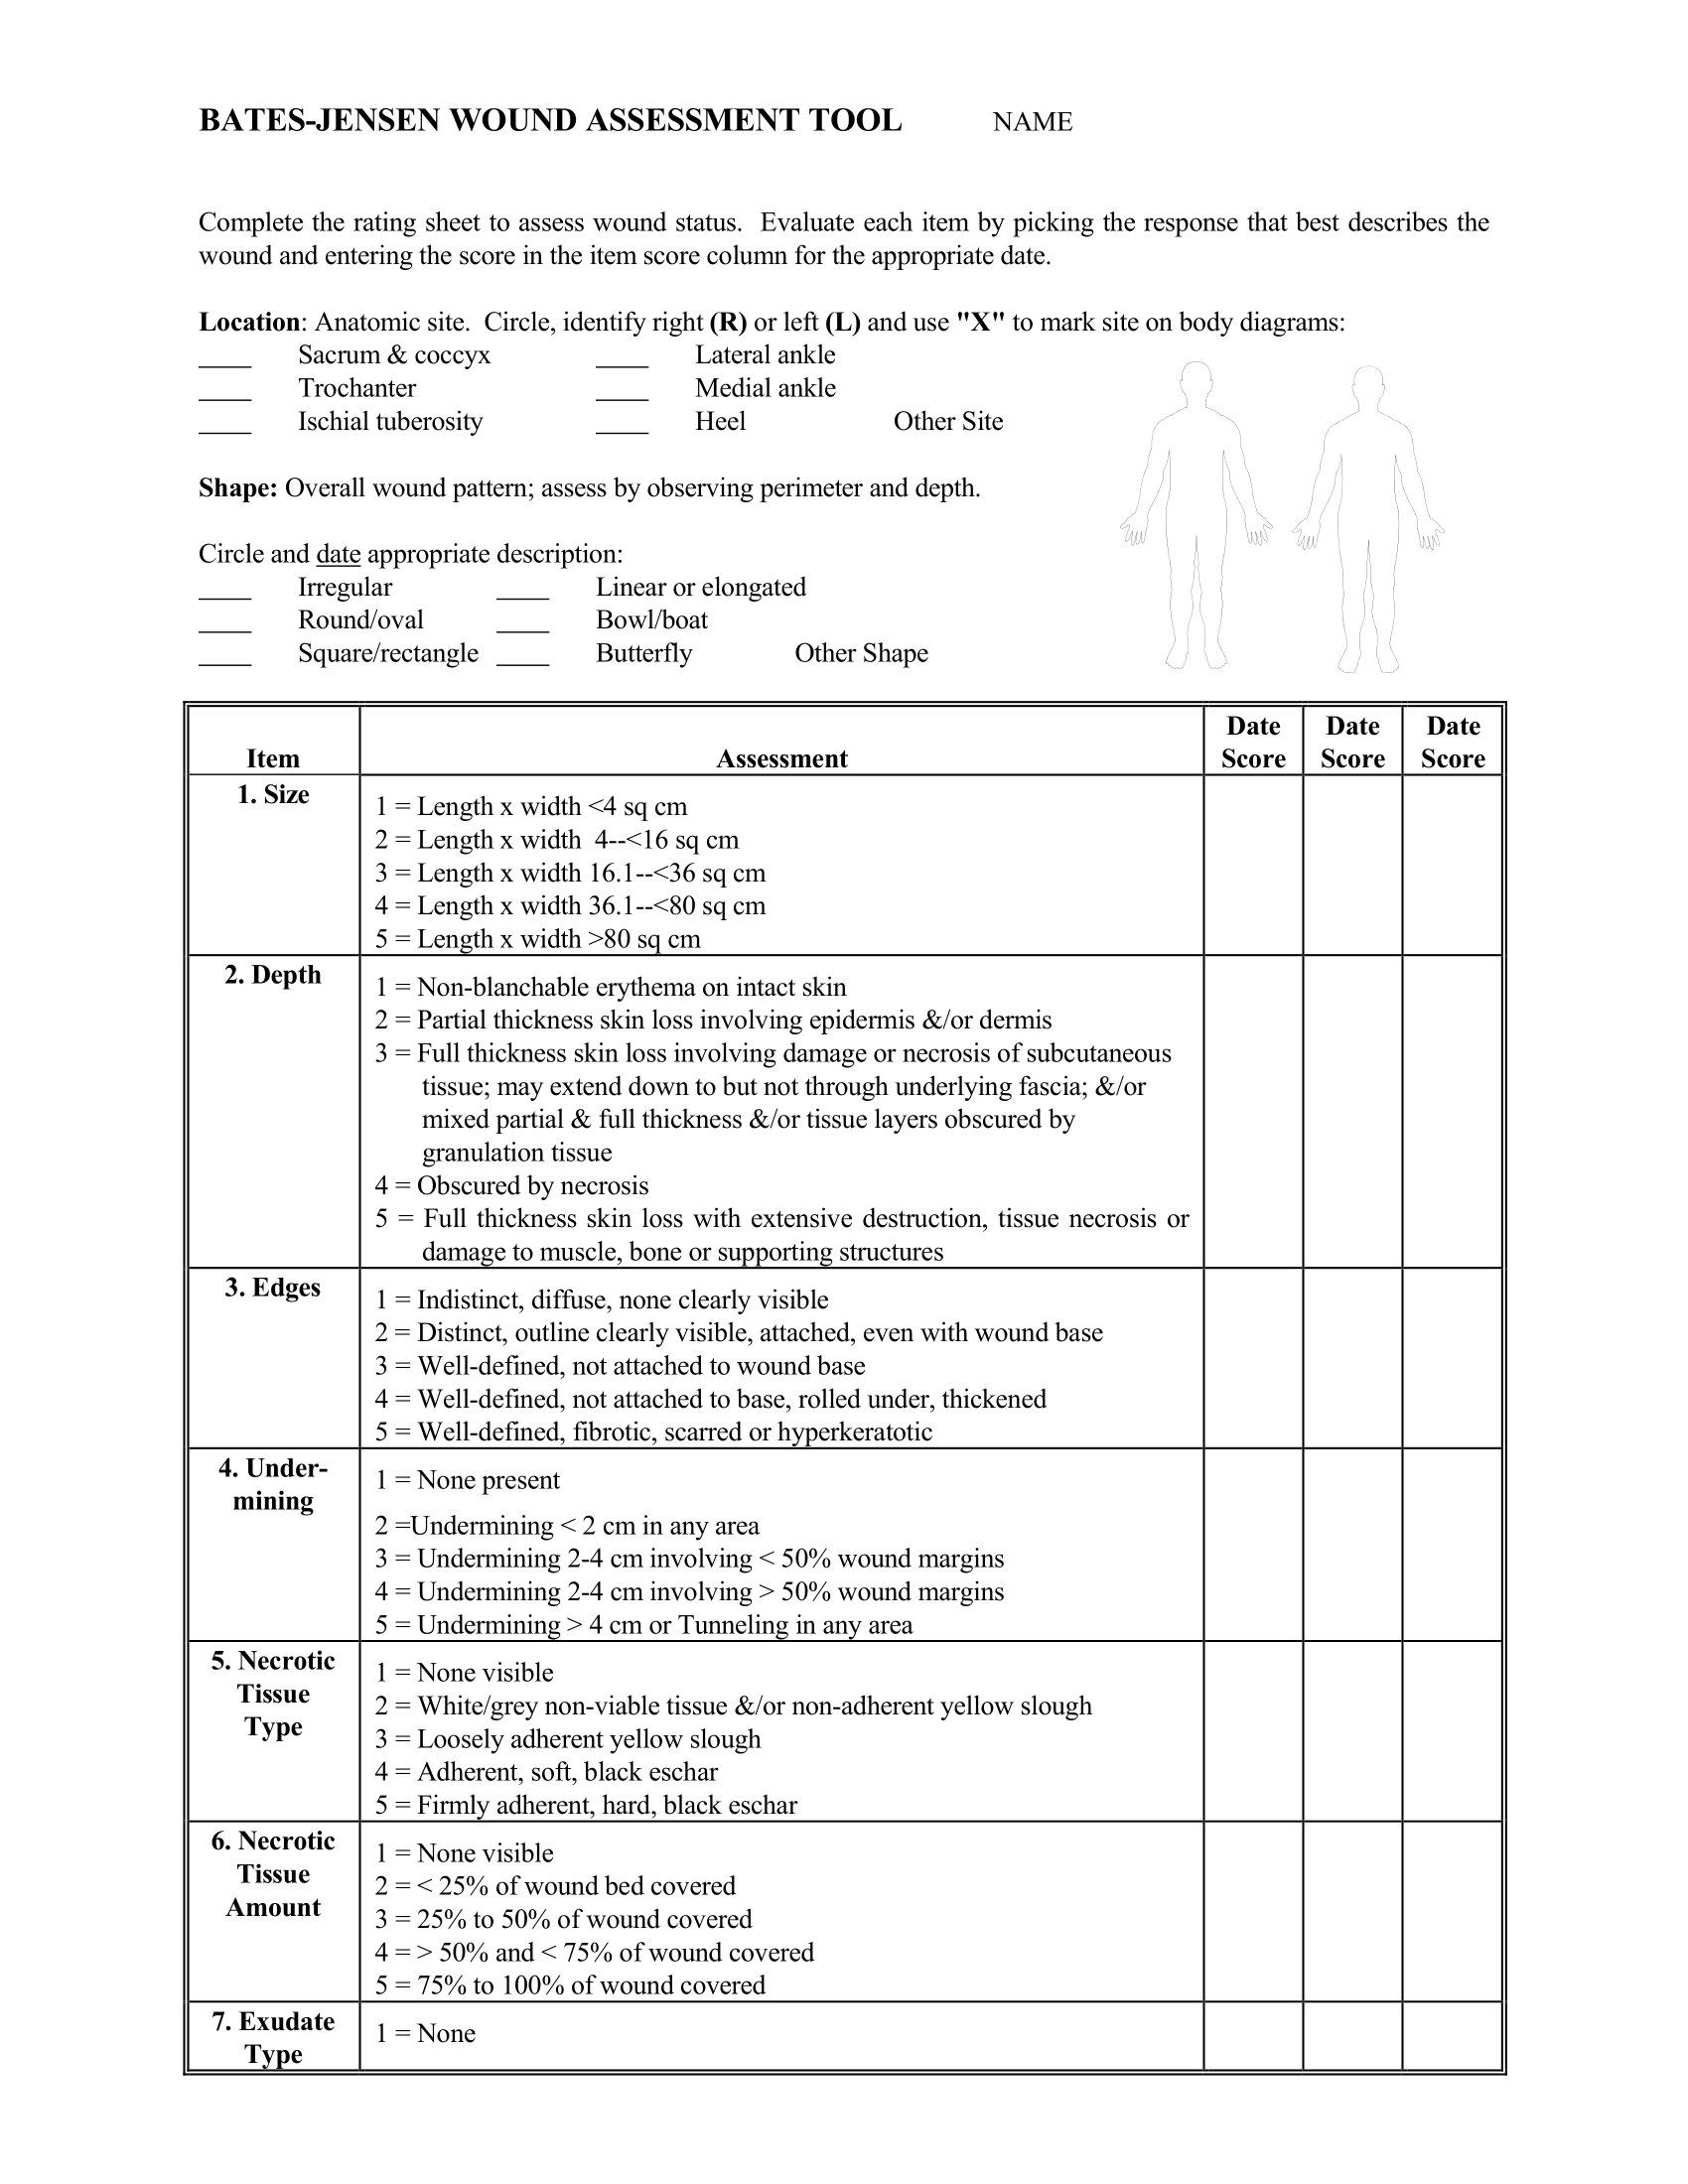
\includegraphics[keepaspectratio, width=14cm]{gambar/BWAT-3}
	\label{gambar:bwat_3}
\end{figure}

\begin{figure}[H]
	\centering
	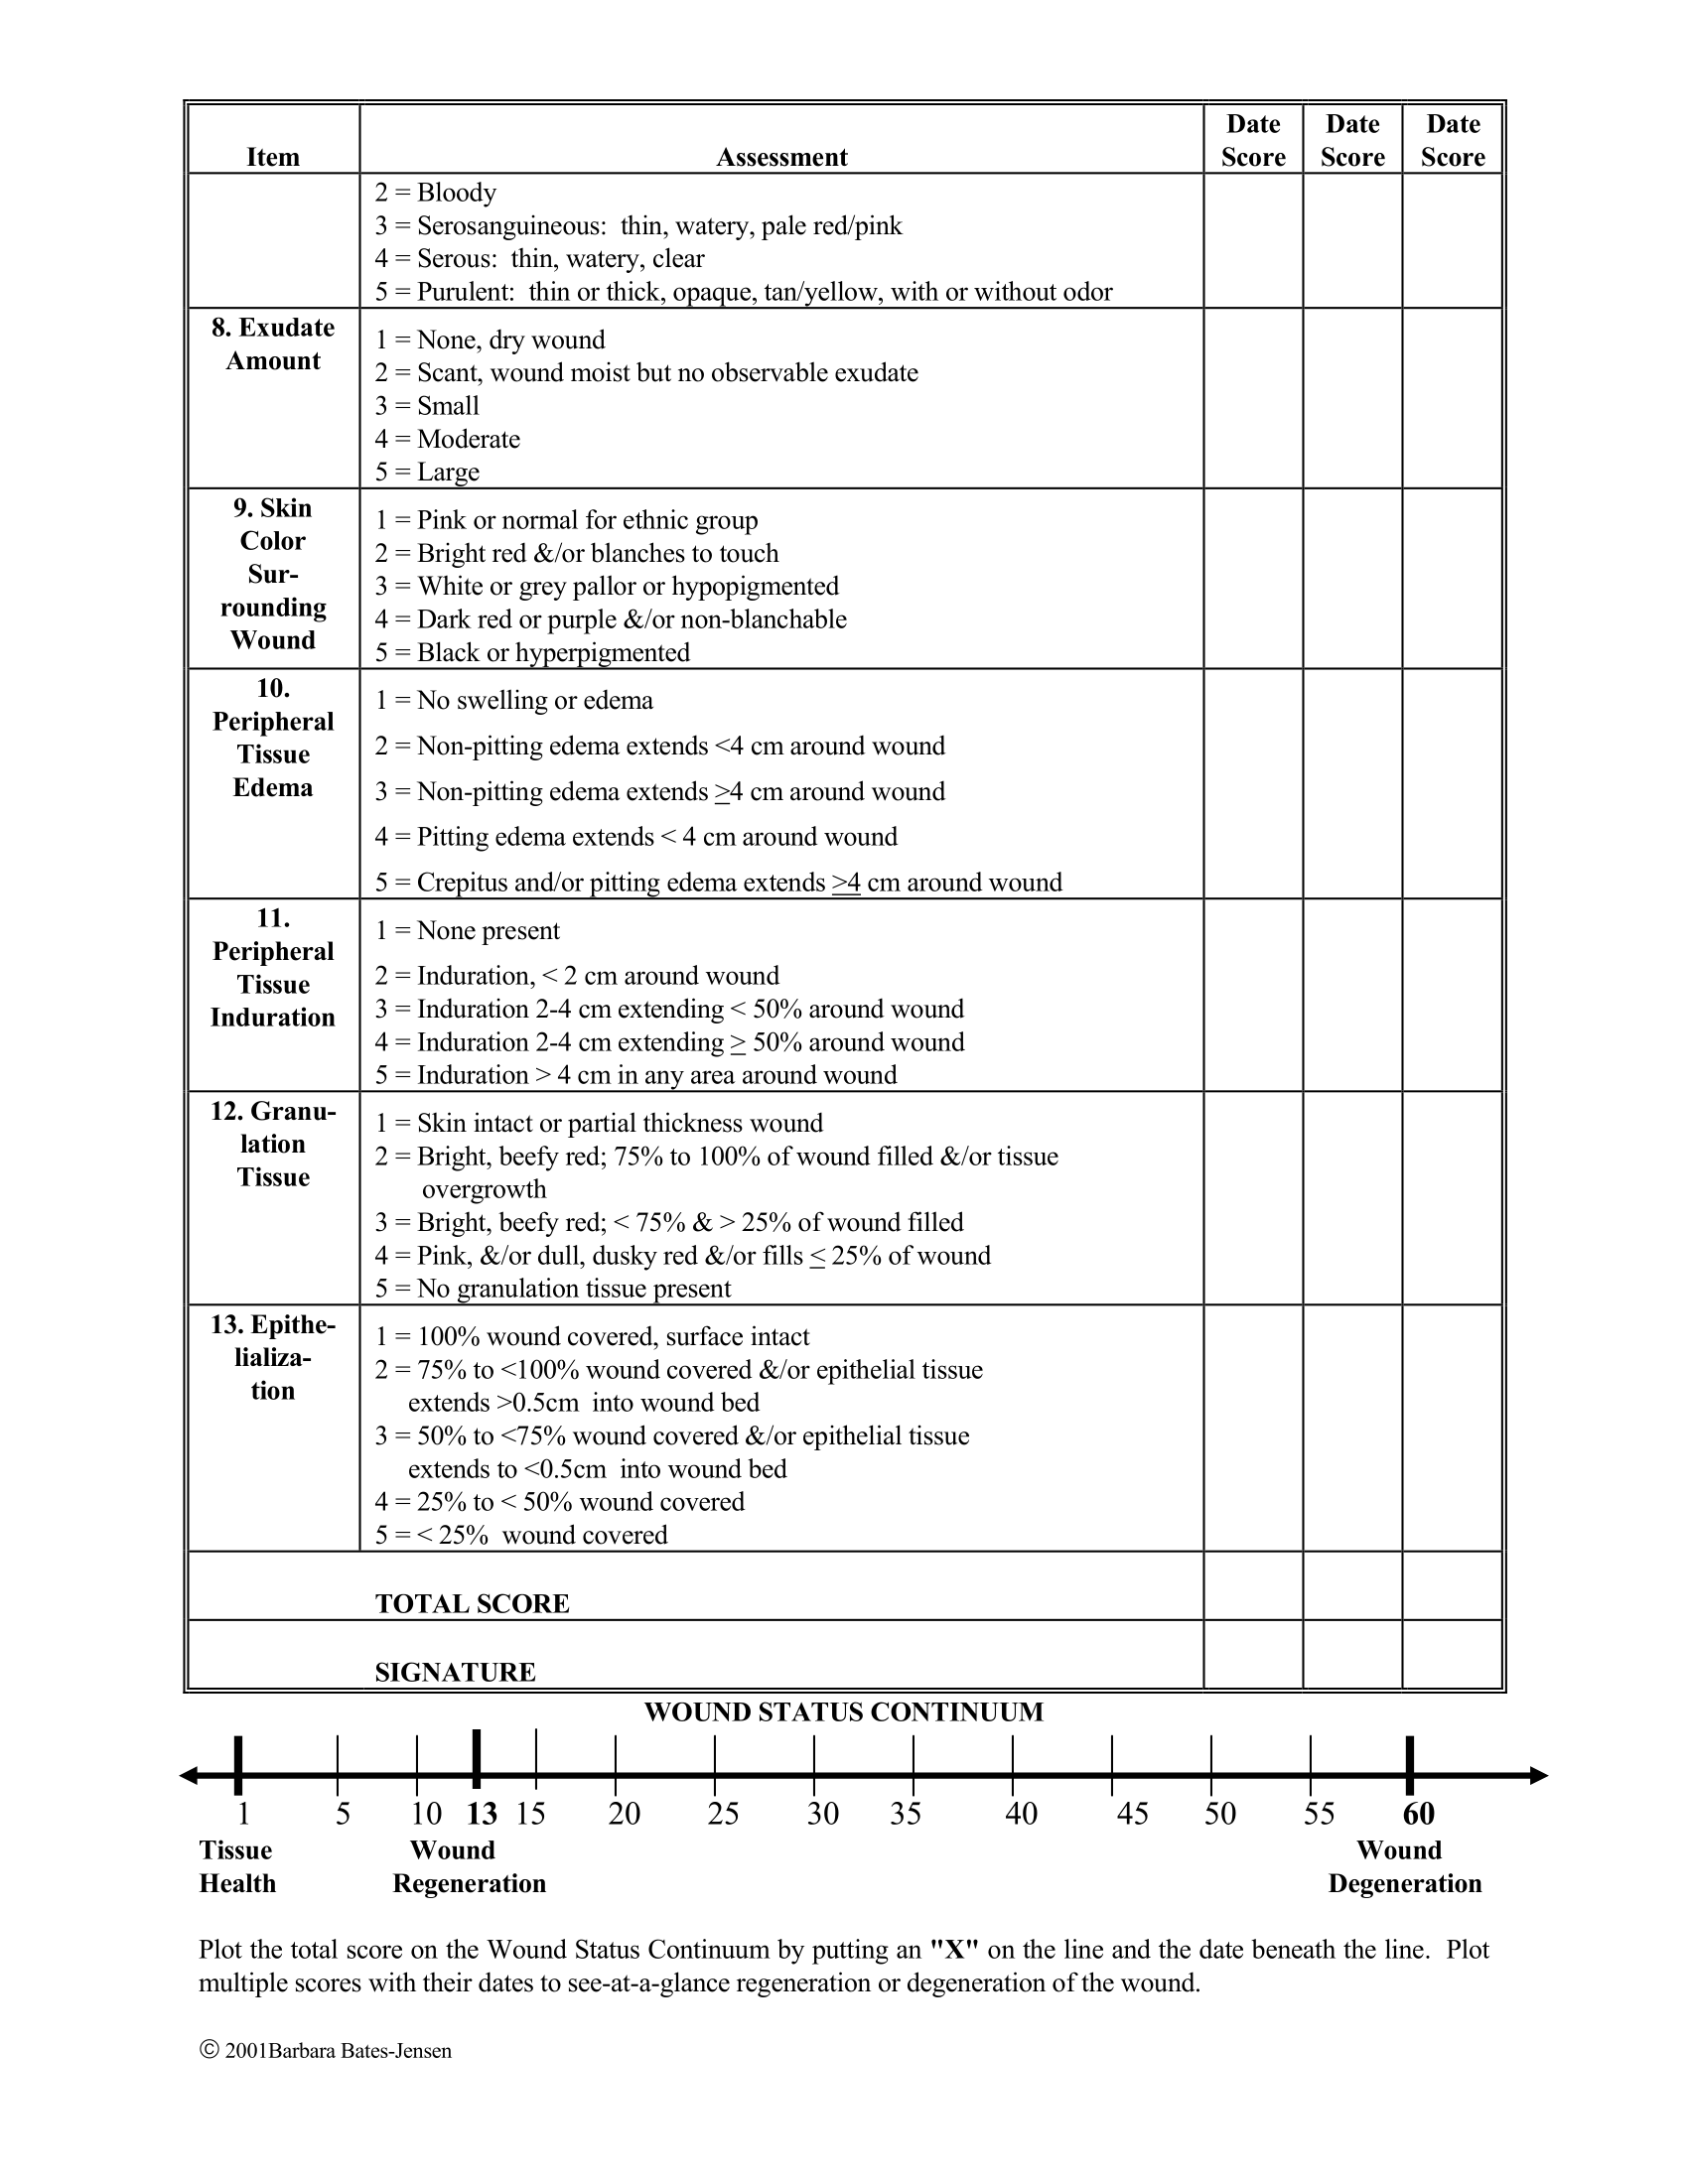
\includegraphics[keepaspectratio, width=14cm]{gambar/BWAT-4}
	\label{gambar:bwat_4}
\end{figure}

\chapter{Format Pengkajian Luka Klinik Moist Care}

\begin{figure}[H]
	\centering
	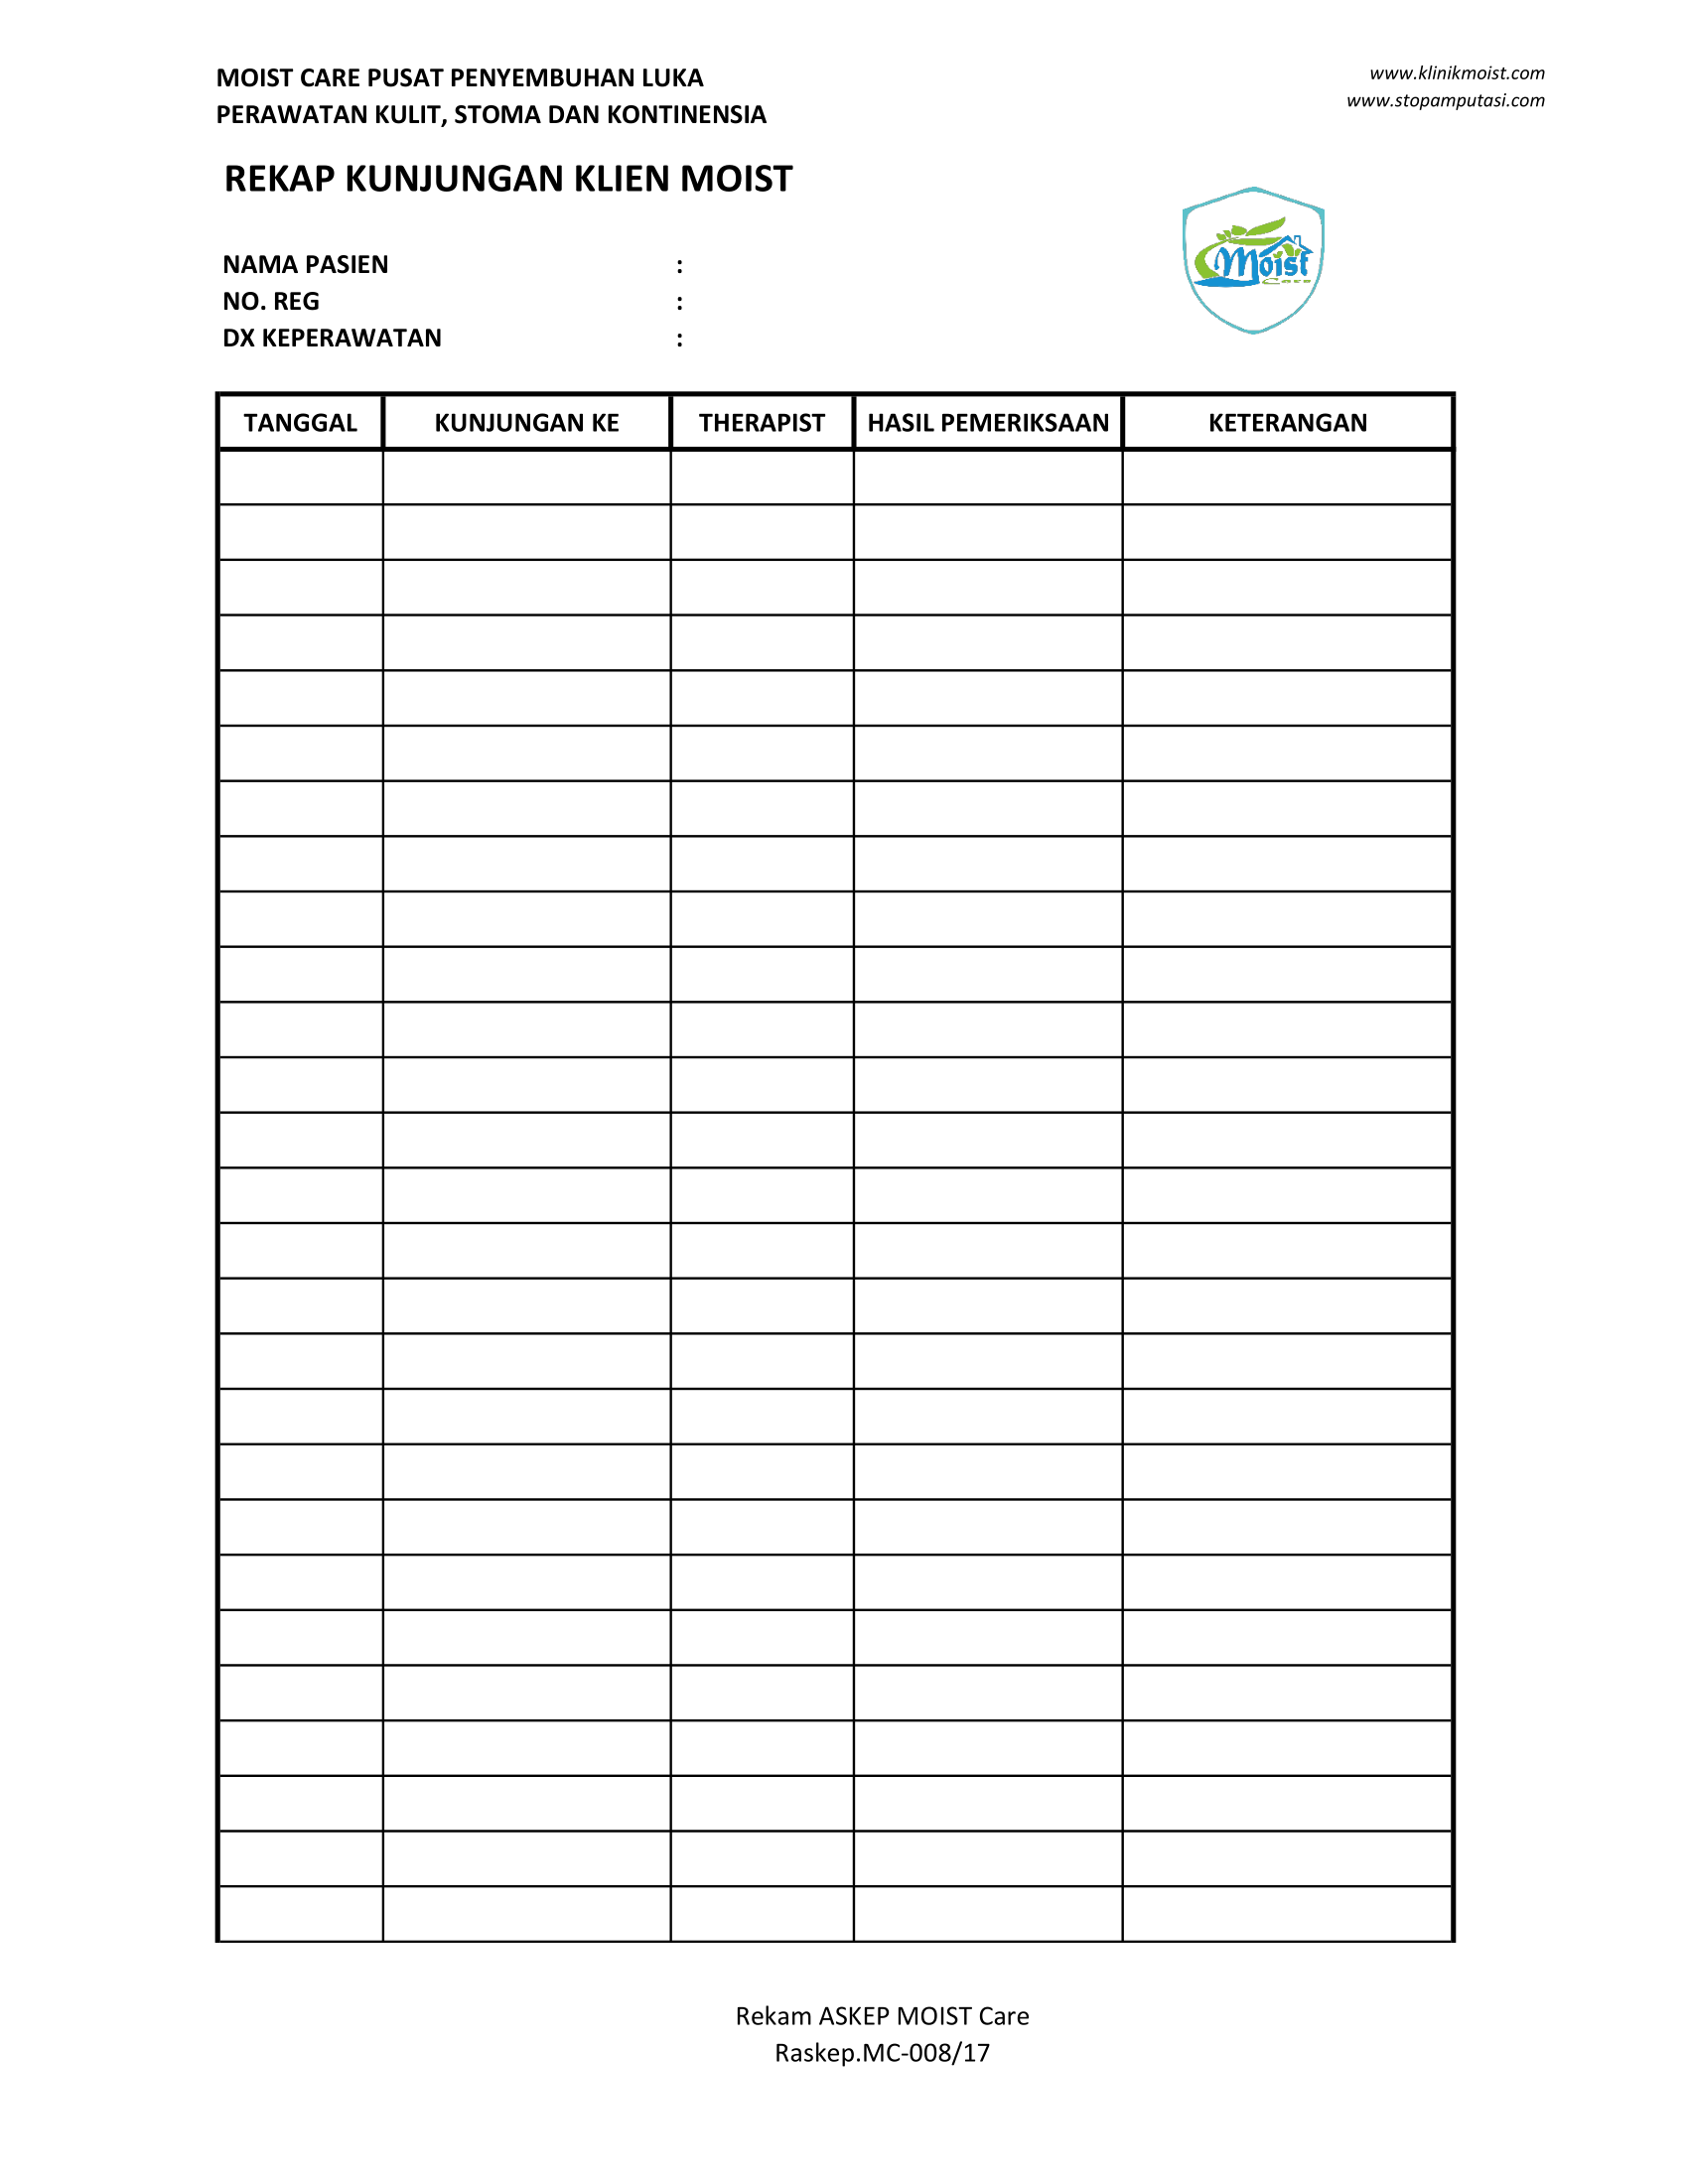
\includegraphics[keepaspectratio, width=14cm]{gambar/Format_Pengkajian-1}
	\label{gambar:Format_Pengkajian_1}
\end{figure}

\begin{figure}[H]
	\centering
	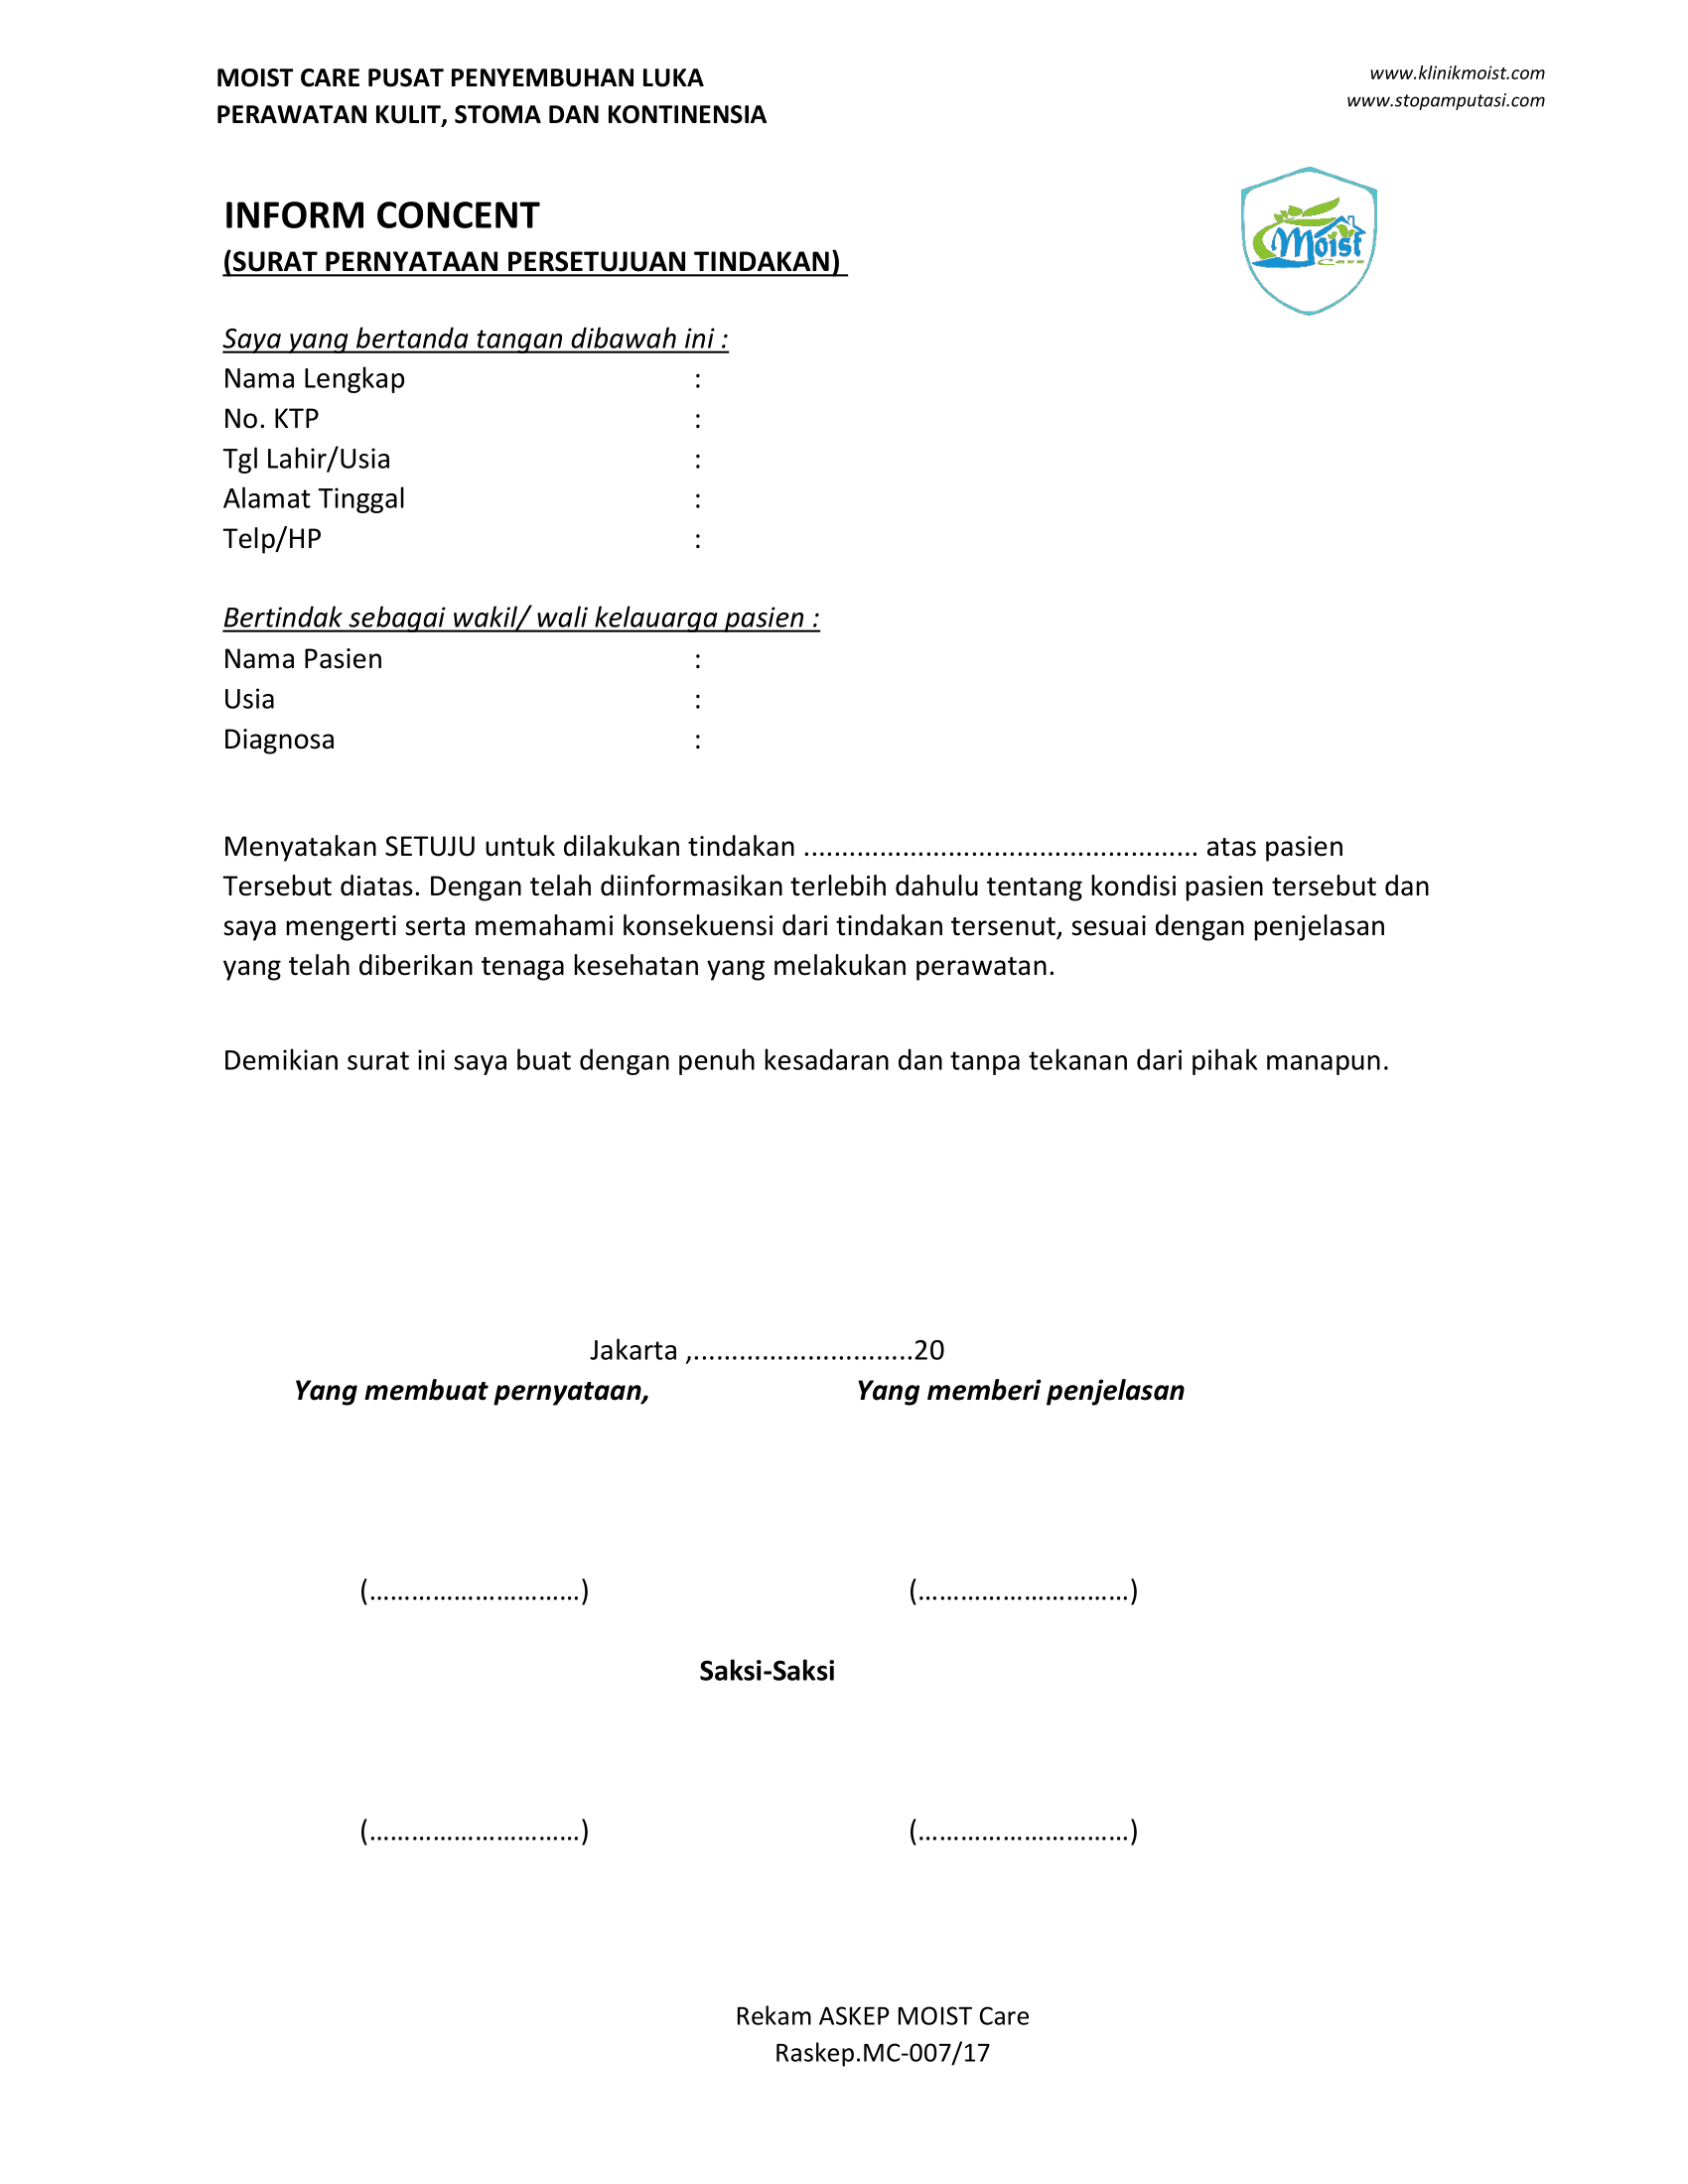
\includegraphics[keepaspectratio, width=14cm]{gambar/Format_Pengkajian-2}
	\label{gambar:Format_Pengkajian_2}
\end{figure}

\begin{figure}[H]
	\centering
	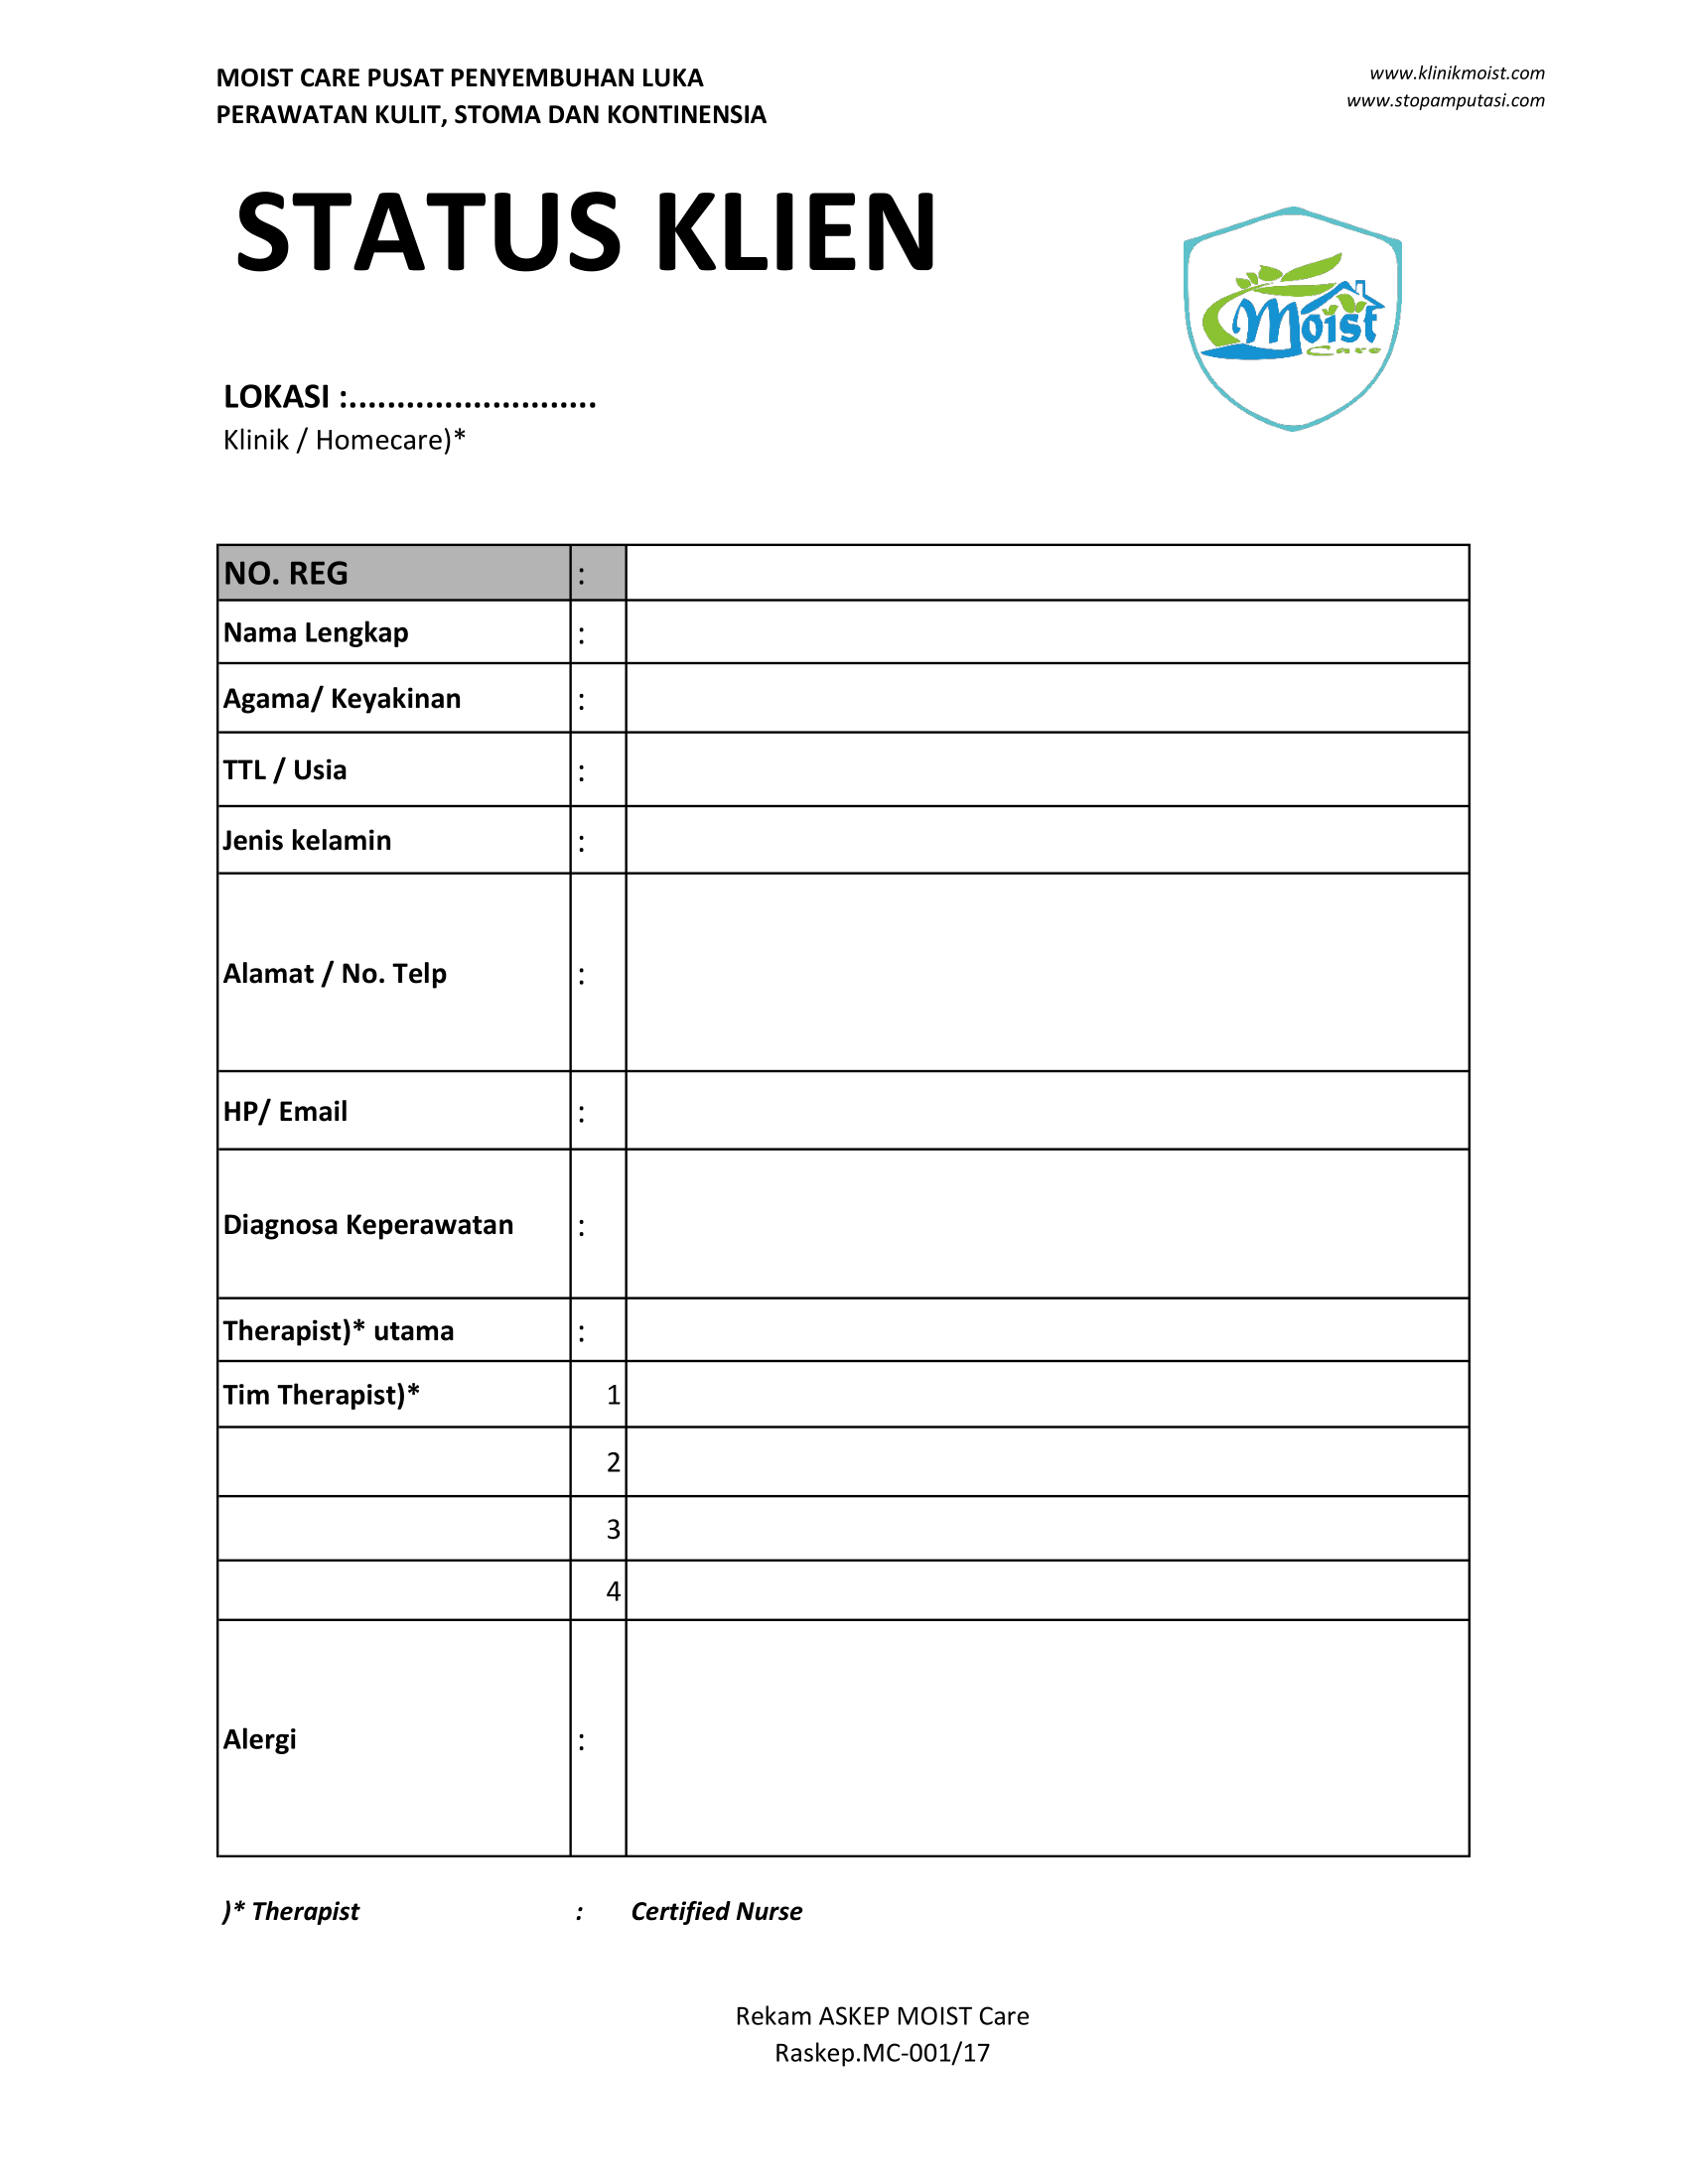
\includegraphics[keepaspectratio, width=14cm]{gambar/Format_Pengkajian-3}
	\label{gambar:Format_Pengkajian_3}
\end{figure}

\begin{figure}[H]
	\centering
	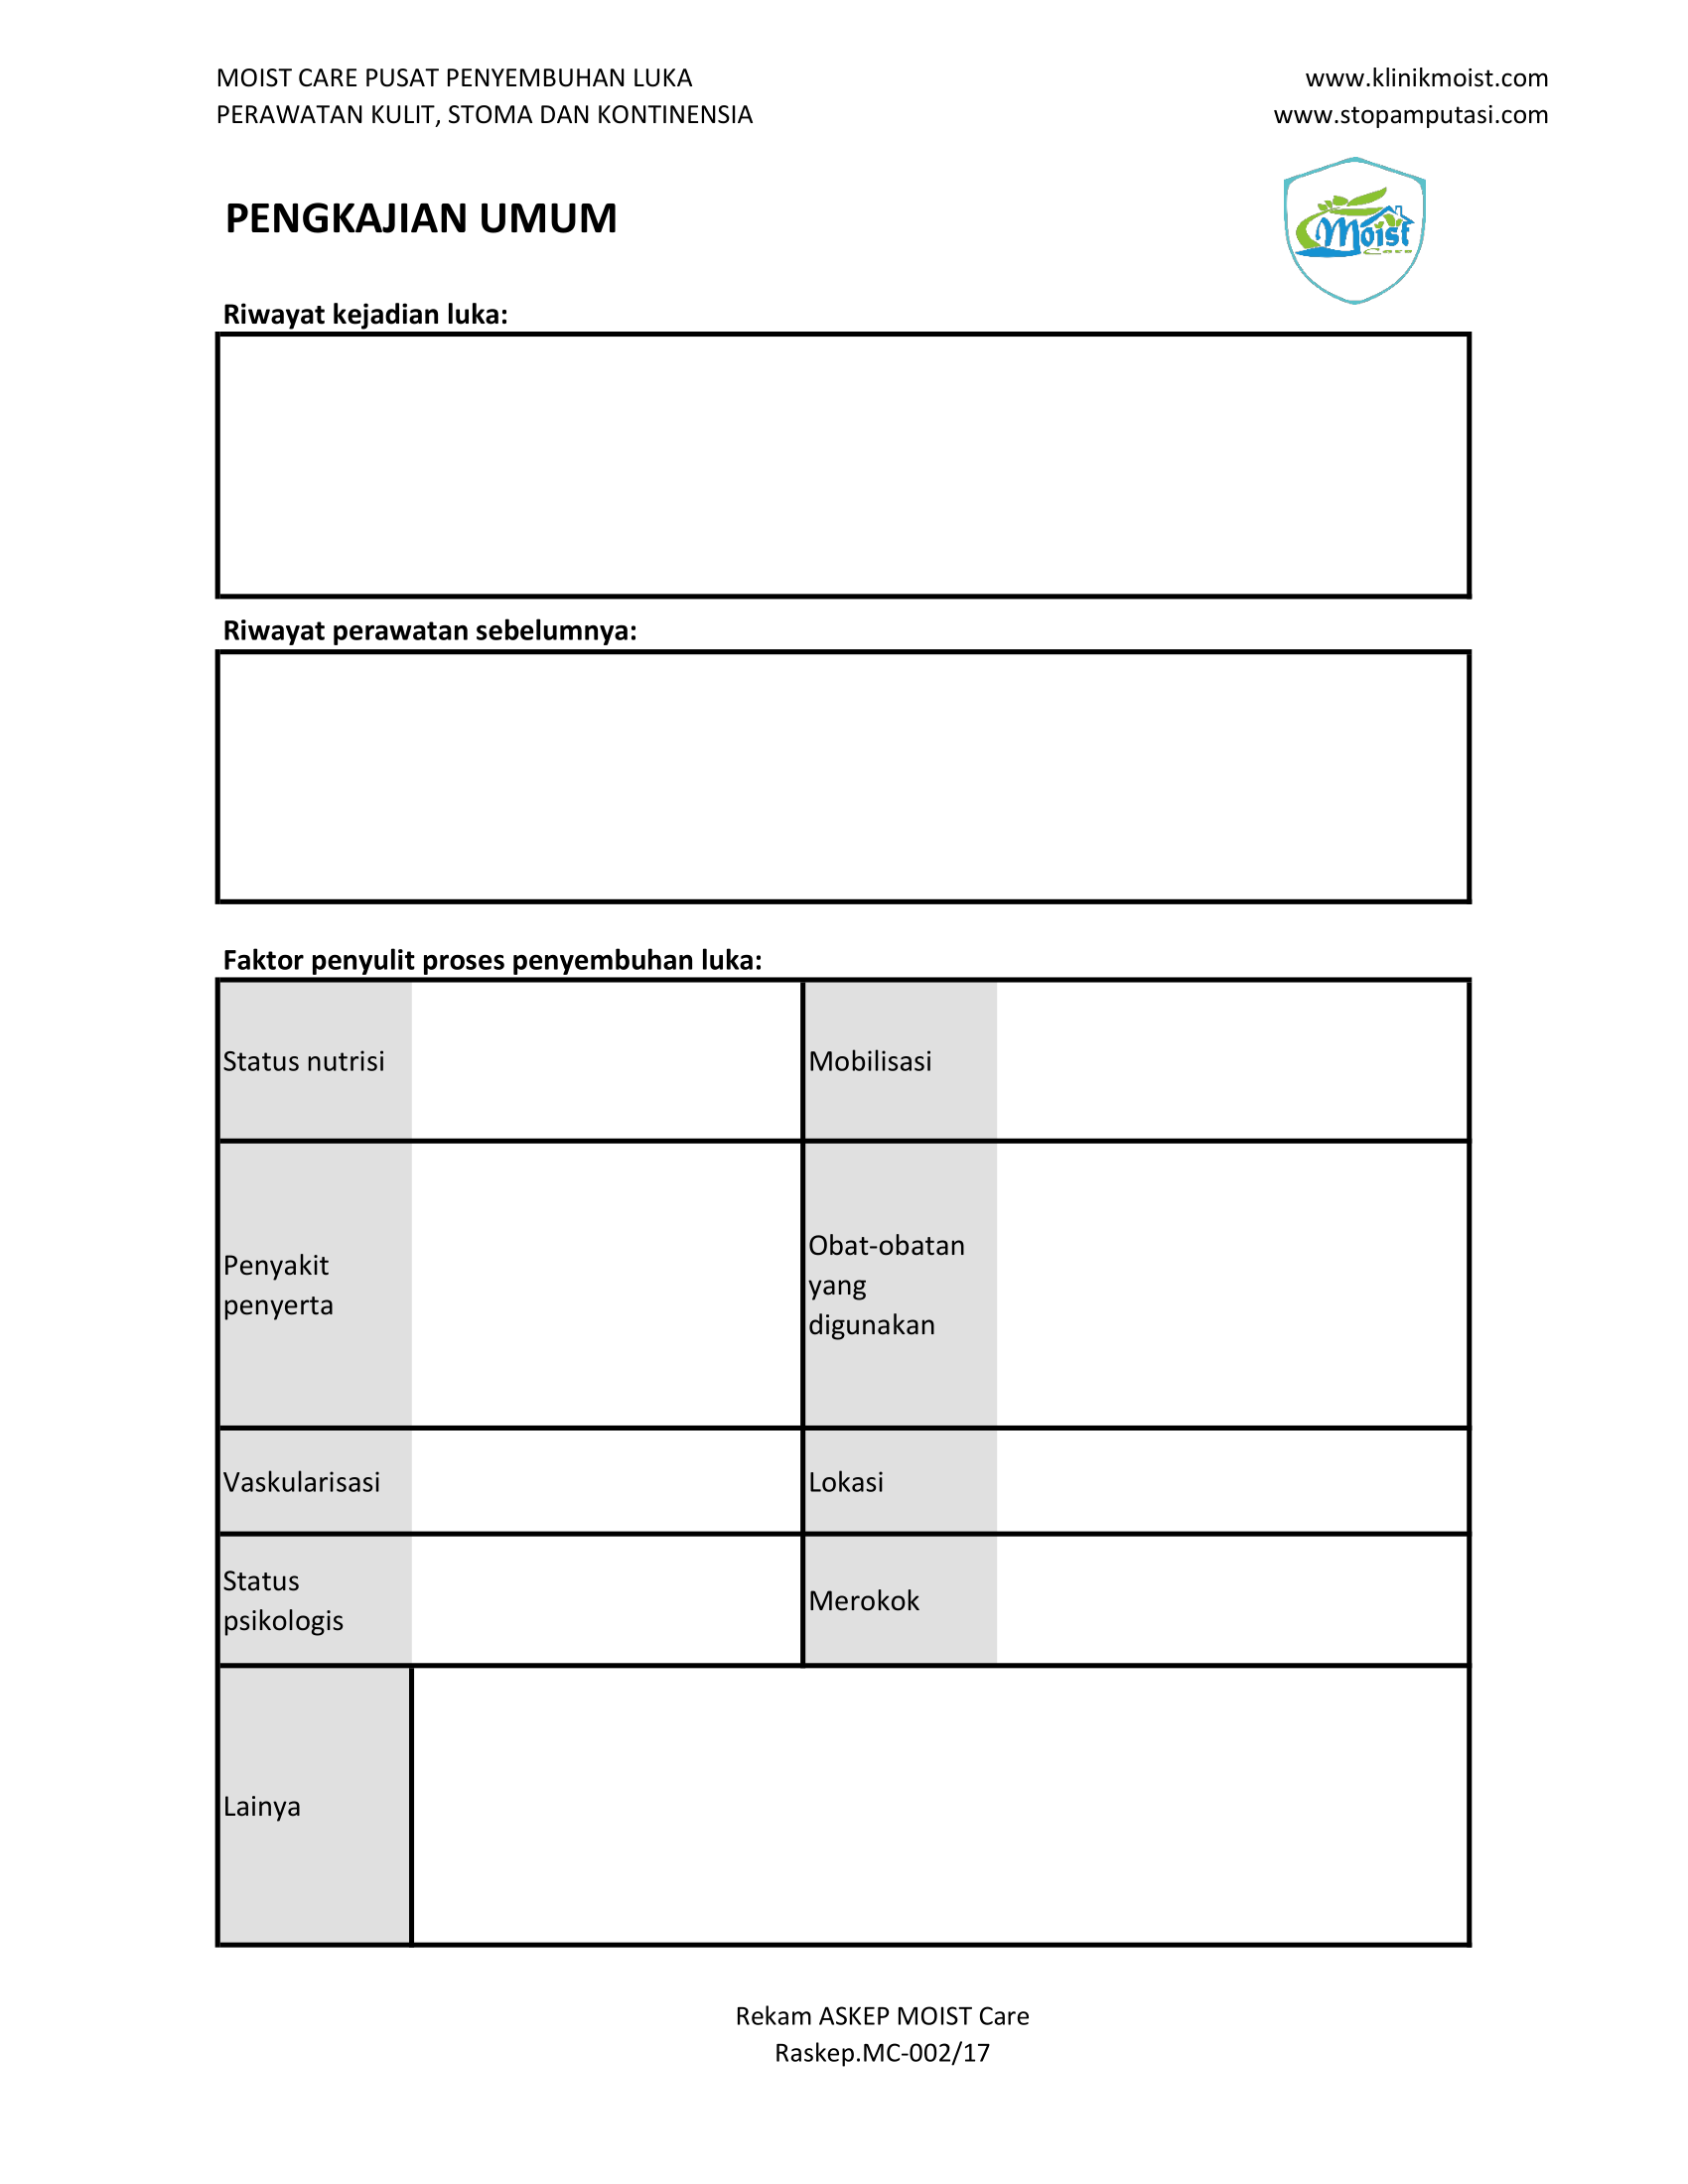
\includegraphics[keepaspectratio, width=14cm]{gambar/Format_Pengkajian-4}
	\label{gambar:Format_Pengkajian_4}
\end{figure}

\begin{figure}[H]
	\centering
	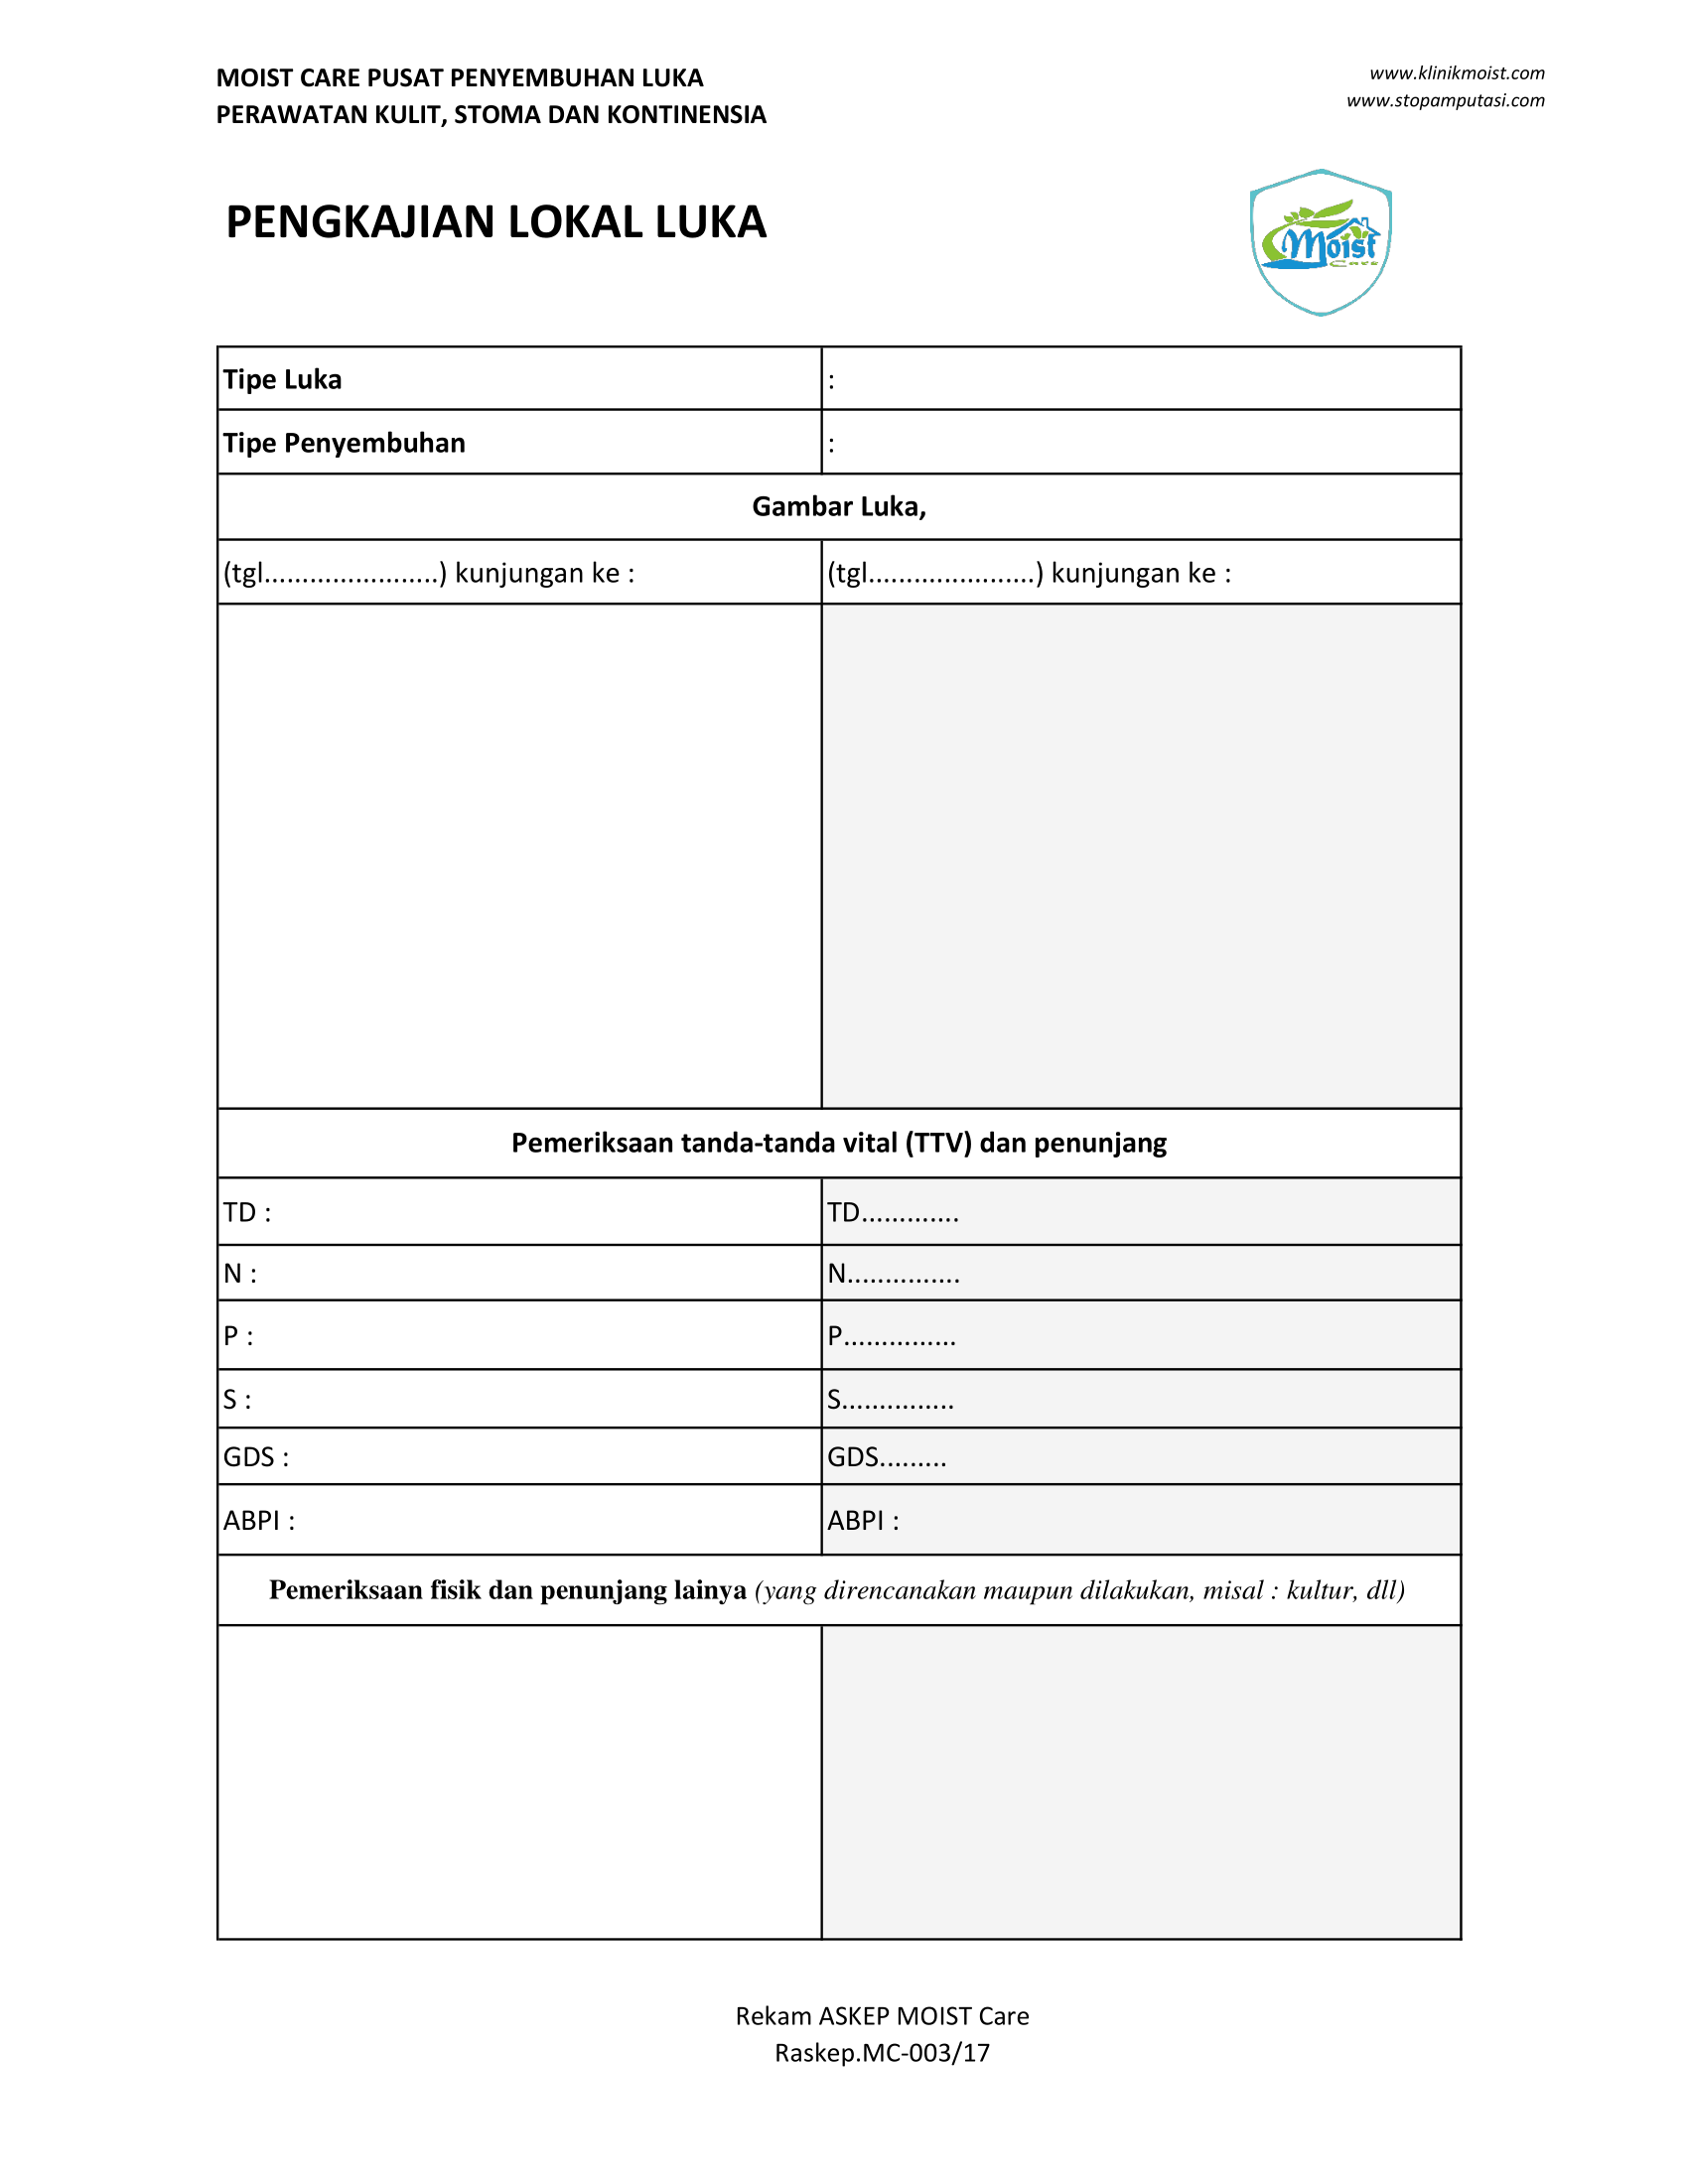
\includegraphics[keepaspectratio, width=14cm]{gambar/Format_Pengkajian-5}
	\label{gambar:Format_Pengkajian_5}
\end{figure}

\begin{figure}[H]
	\centering
	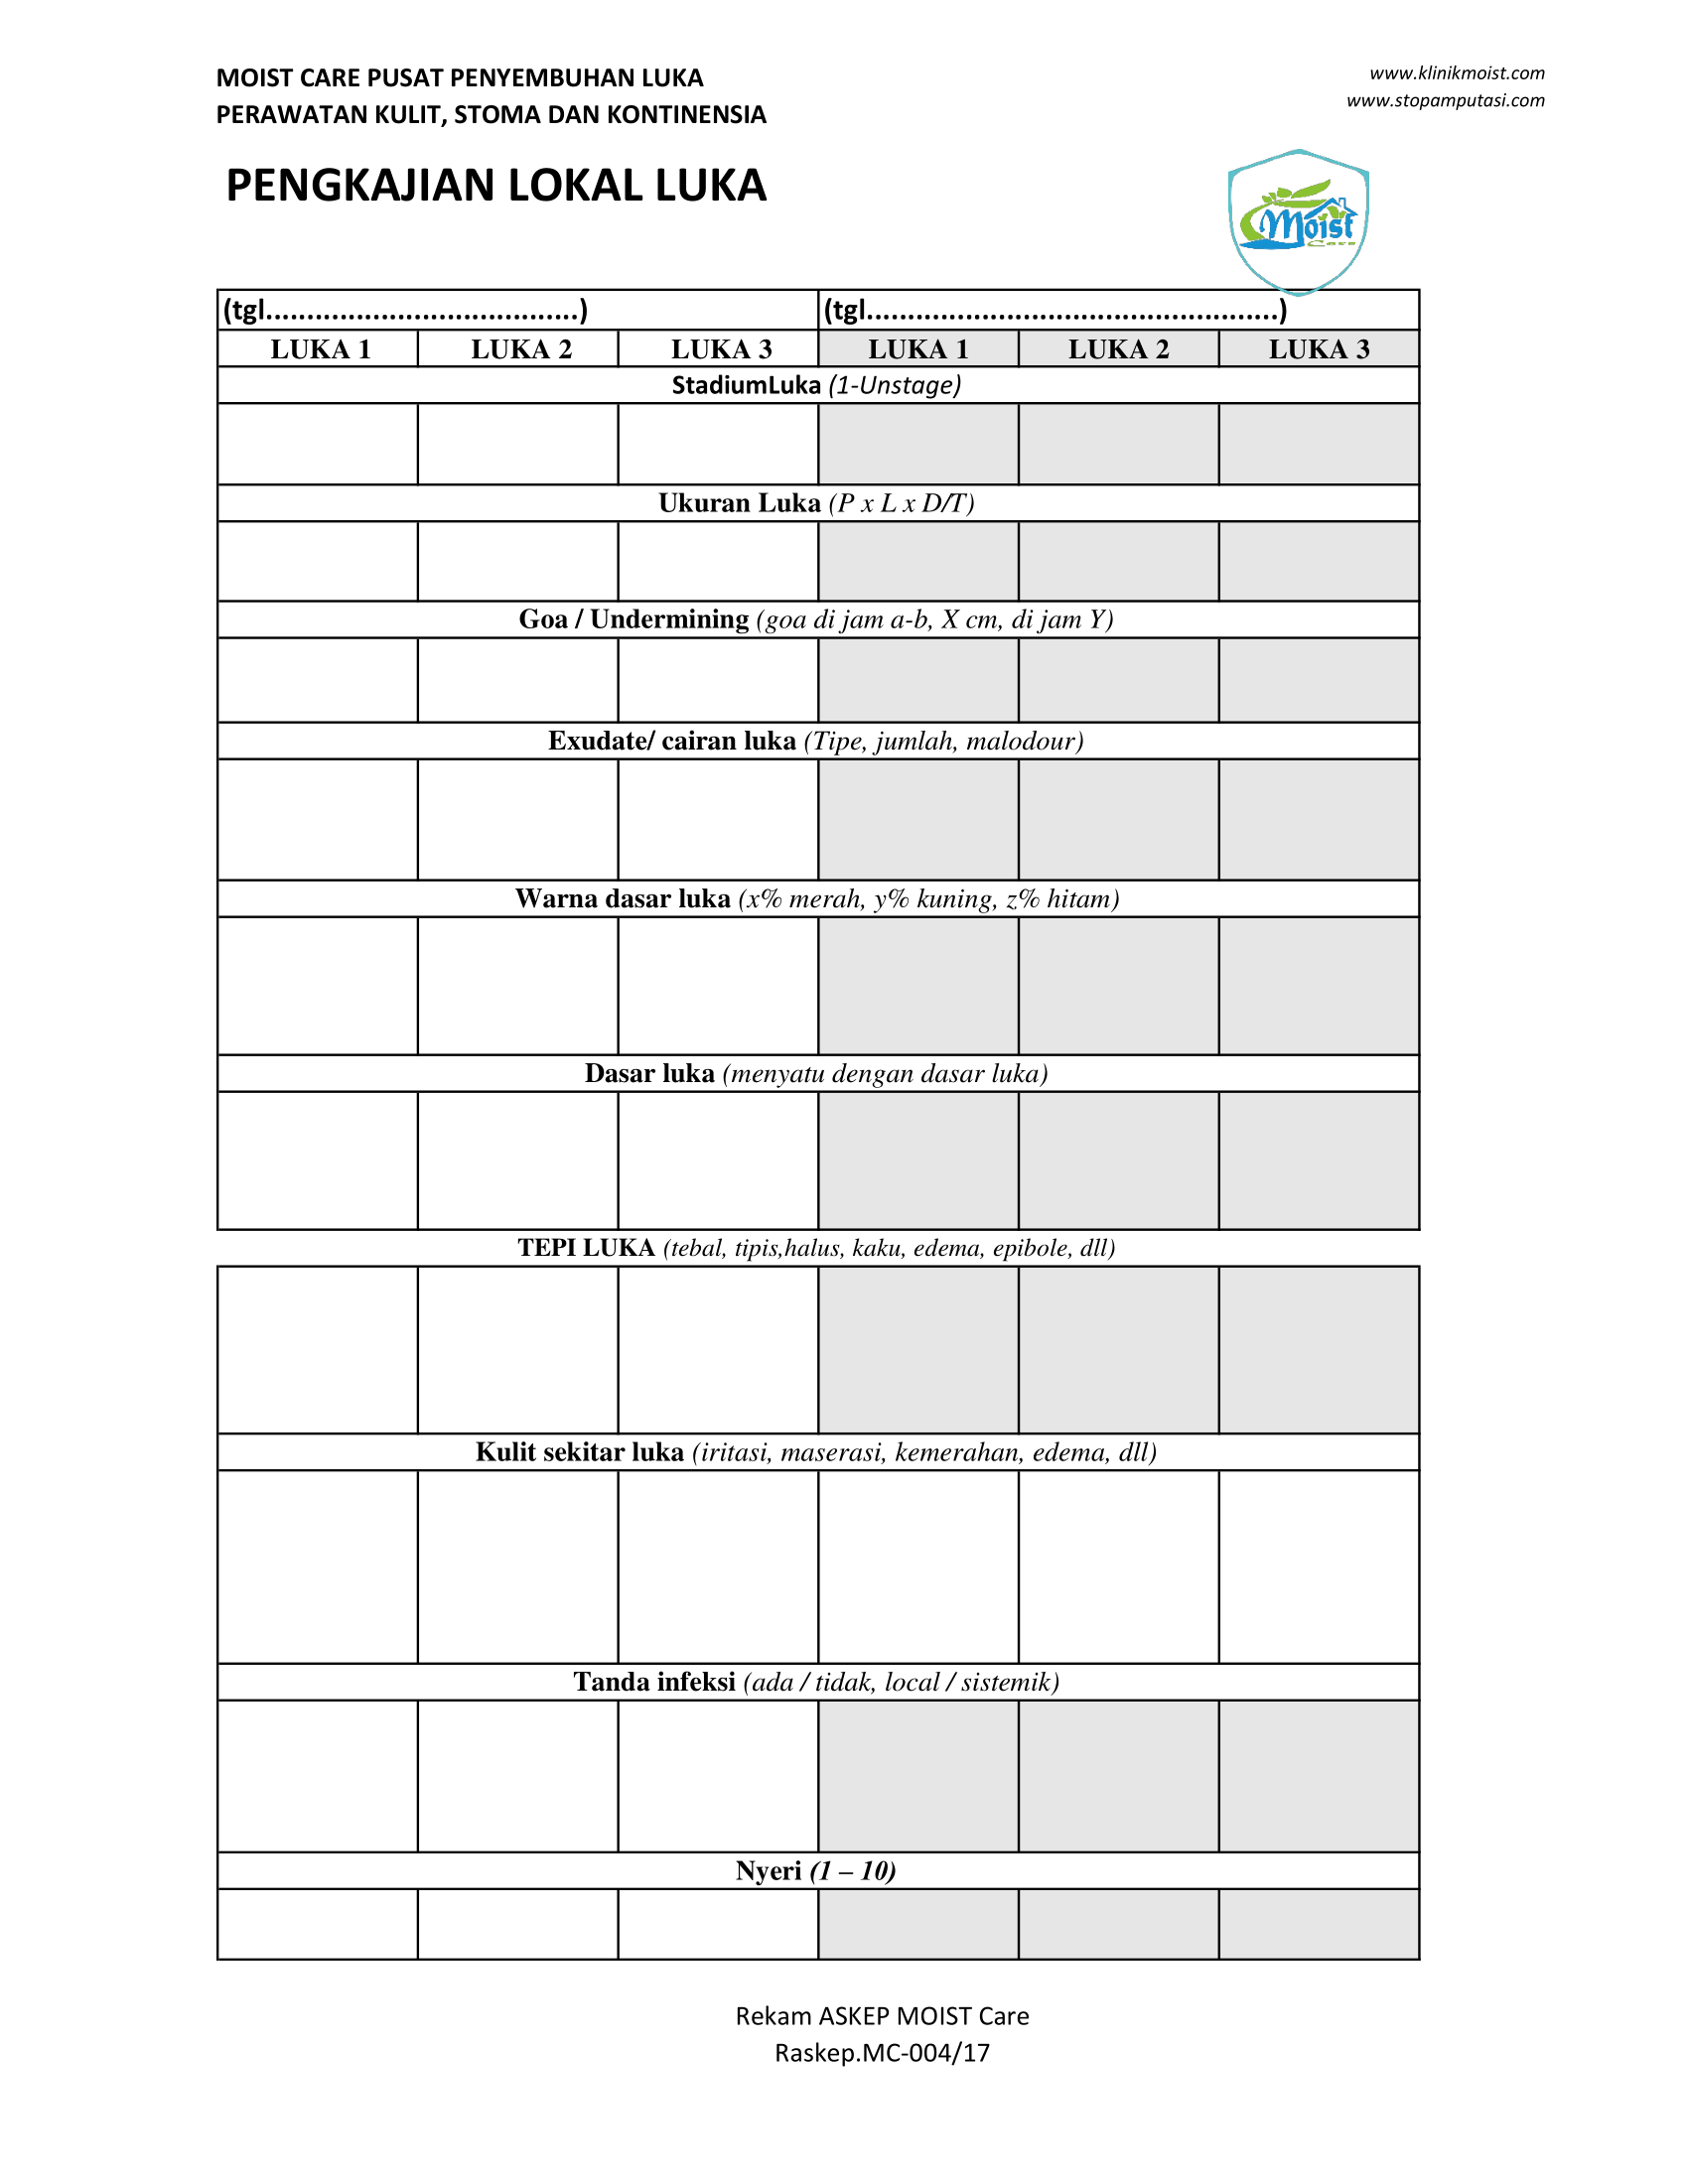
\includegraphics[keepaspectratio, width=14cm]{gambar/Format_Pengkajian-6}
	\label{gambar:Format_Pengkajian_6}
\end{figure}

\begin{figure}[H]
	\centering
	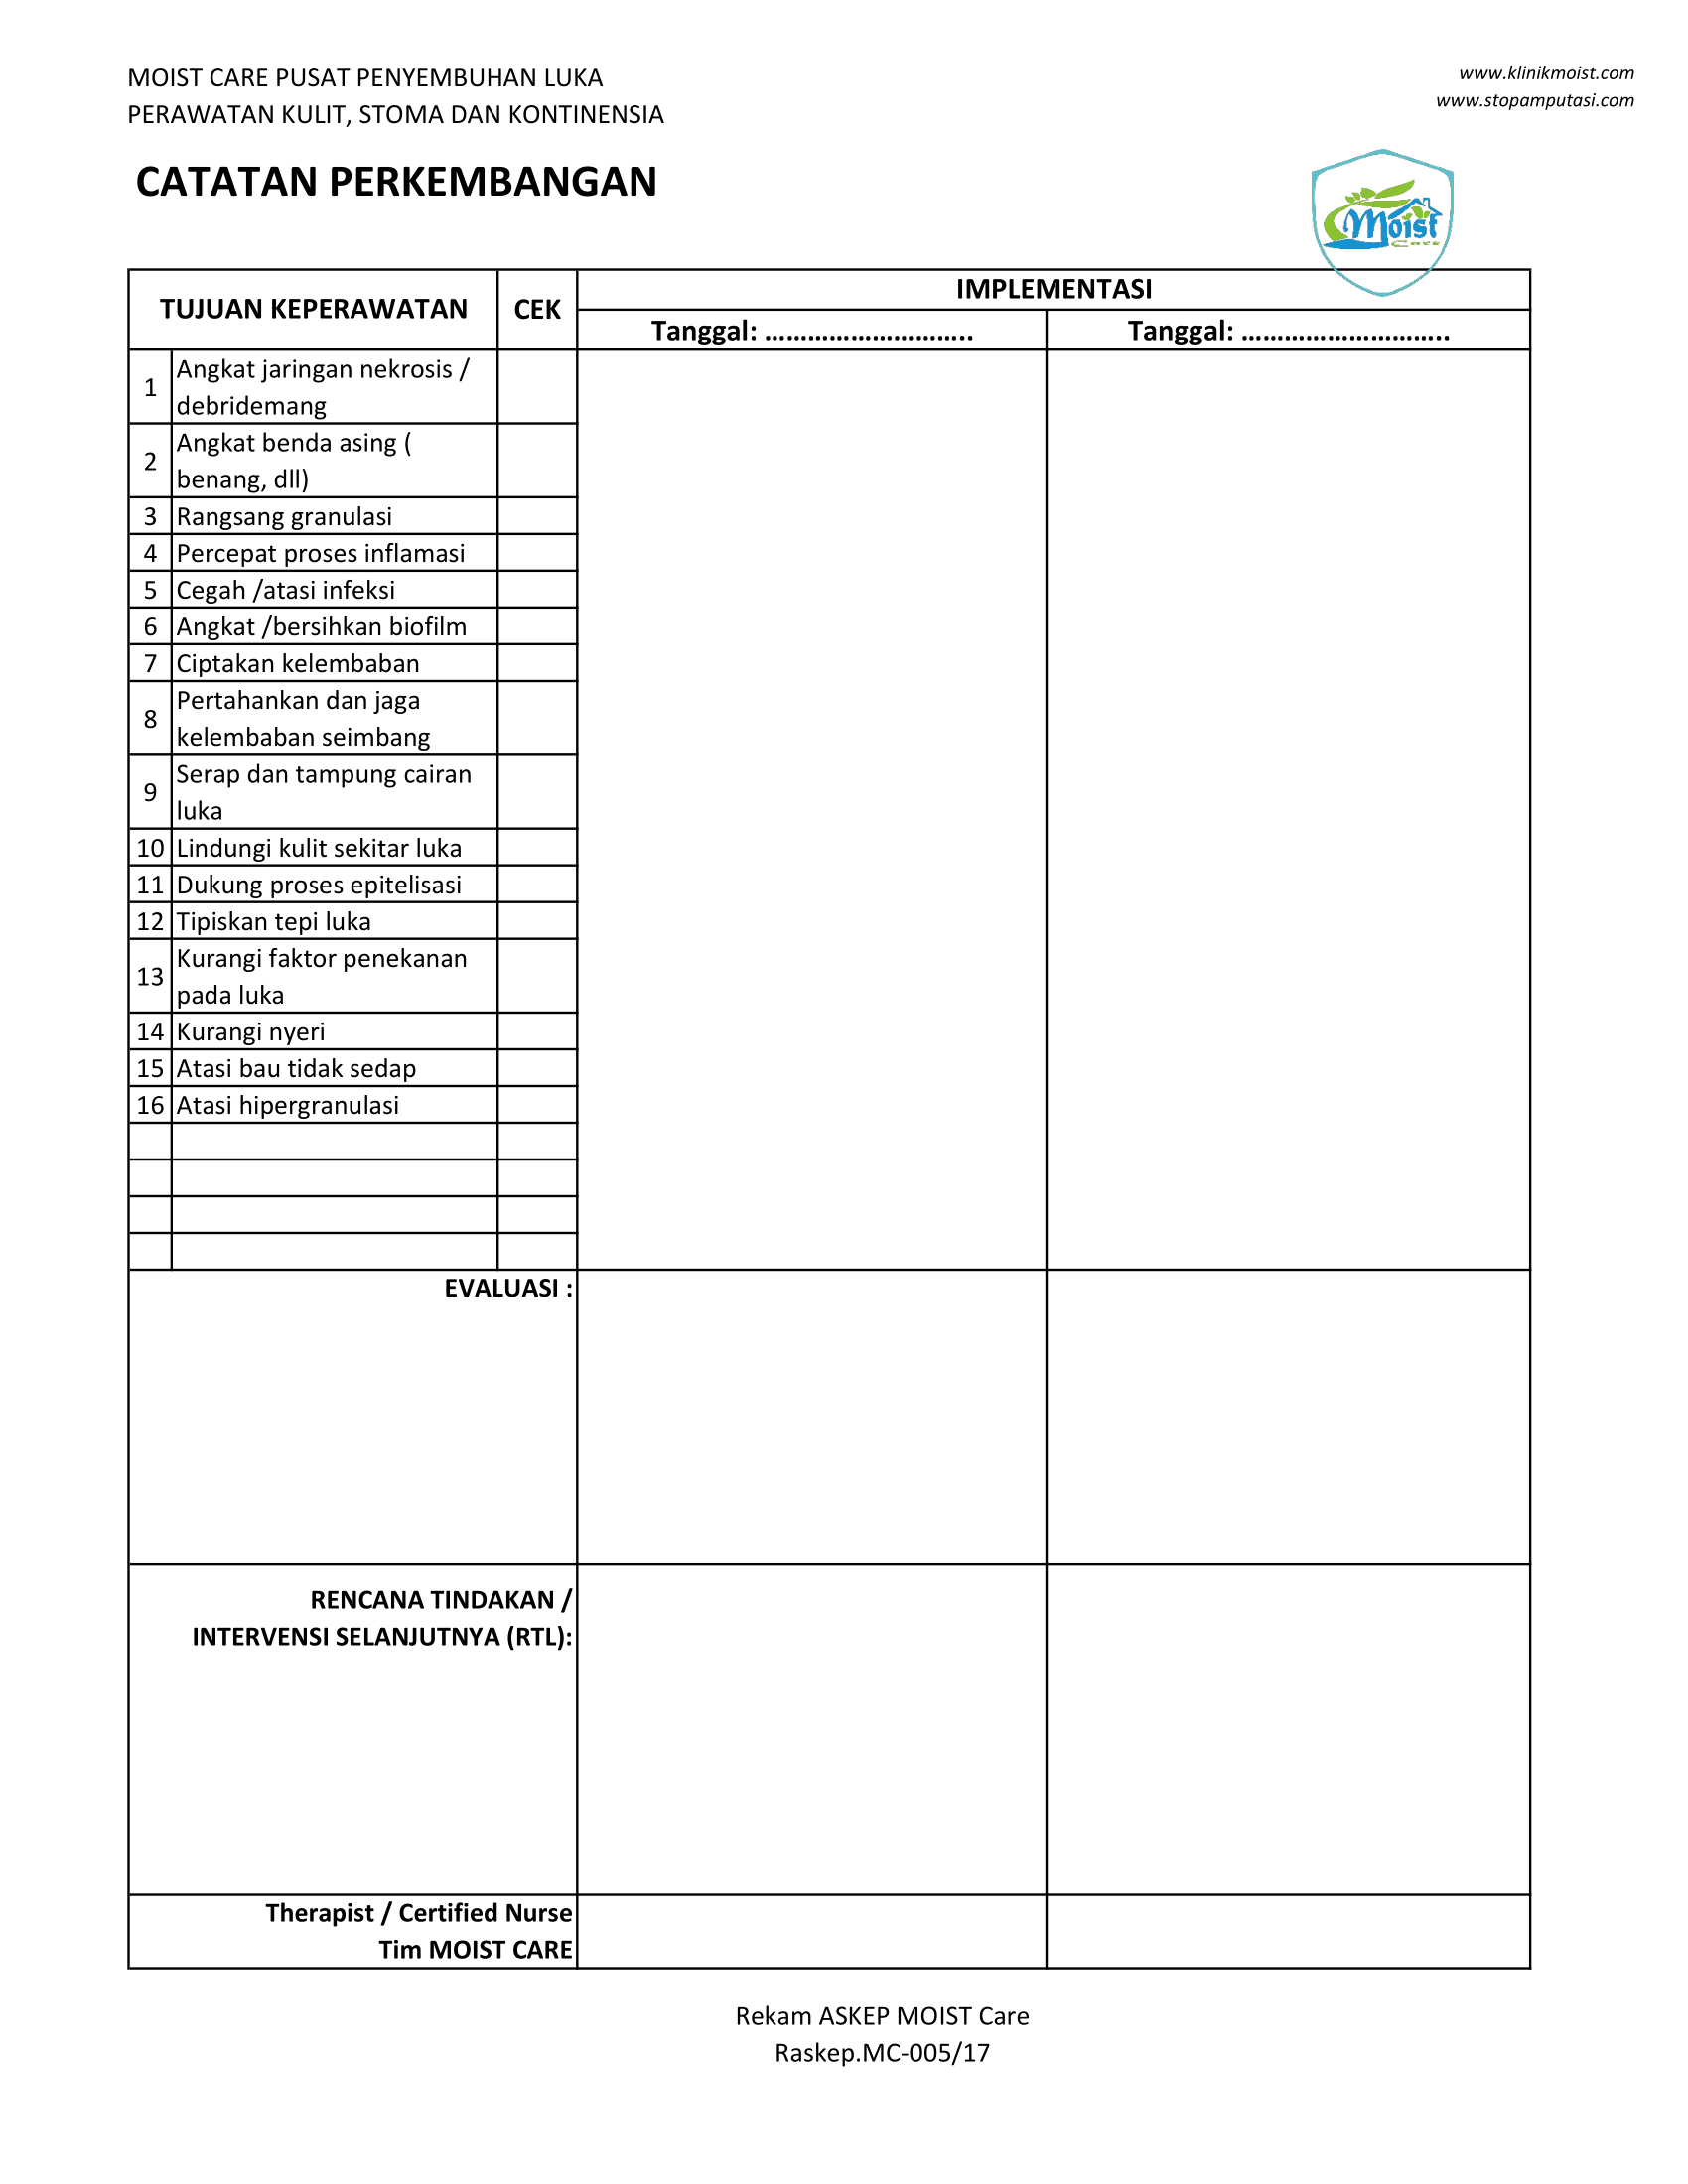
\includegraphics[keepaspectratio, width=14cm]{gambar/Format_Pengkajian-7}
	\label{gambar:Format_Pengkajian_7}
\end{figure}

\chapter{\emph{Source Code}}
\textit{Link github full source code} :
\textit{https://github.com/ardani77/chronic-wound-backend}